%\documentstyle[aas2pp4,epsf]{article}
%%%\documentstyle[aaspp4,epsf]{article}
%\documentstyle[12pt,aasms]{article}    % this is for a preprint
%(single-spaced)
%\documentstyle[aaspp4,epsf]{article} % this is for small print
%\documentstyle[12pt, aaspp4]{article}

%\documentstyle[11pt,aaspp]{article}
%\documentclass[12pt, preprint]{aastex} 

%\documentclass[manuscript]{aastex}
\documentclass[apj]{emulateapj}

%\documentclass[12pt, preprint,numberedappendix]{emulateapj}
%\documentstyle[12pt,aasms]{article}    % this is for submittal
                                       % (double-spaced)

%\documentstyle[12pt,aasms]{article}   \usepackage{emulateapj5} 

\usepackage{graphicx} 
\usepackage{amsmath}
\usepackage{hyperref}
\usepackage{amsfonts}
\usepackage{amsmath}
\usepackage{amssymb}
\usepackage{amsthm}
\usepackage{subeqnarray}
\usepackage{ulem}
%\bibliographystyle{apj}

\newcommand{\delad}{\nabla_{\rm ad}}
\newcommand{\delrad}{\nabla_{\rm rad}}
\newcommand{\emgr}[1]{\emph{ \color{gray} #1}}

\newcommand{\ie}{i.e.\ }
\newcommand{\eg}{e.g.\ }
\newcommand{\p}{\partial}
\newcommand{\xv}{\vc{x}}
\newcommand{\kv}{\vc{k}}
\newcommand{\brak}[1]{\langle #1\rangle}


\newcommand{\gcc}{\;\mathrm{g\; cm^{-3}}}
\newcommand{\gsc}{\;\mathrm{g\; cm^{-2}}}
\newcommand{\cm}{\; {\rm cm}}
\newcommand{\mm}{\; {\rm mm}}
%\newcommand{\ps}{\; {\rm s^{-1}}}
\newcommand{\km}{\; {\rm km}}
%\newcommand{\au}{\; \varpi_{\rm AU}}

\newcommand{\AU}{\; {\rm AU}}
\newcommand{\yr}{\; {\rm yr}}
\def\K{\; {\rm K}}

\newcommand{\vcs}[1]{\mbox{\boldmath{$\scriptstyle{#1}$}}}
\newcommand{\vc}[1]{\mbox{\boldmath{$#1$}}}
\newcommand{\nab}{\vc{\nabla}}
\DeclareMathSymbol{\varOmega}{\mathord}{letters}{"0A}
\DeclareMathSymbol{\varSigma}{\mathord}{letters}{"06}
\DeclareMathSymbol{\varPsi}{\mathord}{letters}{"09}

\newcommand{\Eq}[1]{Equation\,(\ref{#1})}
\newcommand{\Eqs}[2]{Equations (\ref{#1}) and~(\ref{#2})}
\newcommand{\Eqss}[2]{Equations (\ref{#1})--(\ref{#2})}
\newcommand{\Eqsss}[3]{Equations (\ref{#1}), (\ref{#2}) and~(\ref{#3})}
\newcommand{\App}[1]{Appendix~\ref{#1}}
\newcommand{\Sec}[1]{Sect.~\ref{#1}}
\newcommand{\Chap}[1]{Chapter~\ref{#1}}
\newcommand{\Fig}[1]{Fig.~\ref{#1}}
\newcommand{\Figs}[2]{Figs.~\ref{#1} and \ref{#2}}
\newcommand{\Figss}[2]{Figs.~\ref{#1}--\ref{#2}} 
\newcommand{\Tab}[1]{Table \ref{#1}}

\newenvironment{packed_item}{
\begin{itemize}
  \setlength{\itemsep}{1pt}
  \setlength{\parskip}{0pt}
  \setlength{\parsep}{0pt}
}{\end{itemize}}

%\newcommand{\delad}{\nabla_{\rm ad}}
%\newcommand{\delrad}{\nabla_{\rm rad}}
\newcommand{\Rg}{\mathcal{R}}
\newcommand{\RB}{R_{\rm B}}
\newcommand{\co}{_{\rm c}}
\newcommand{\di}{_{\rm d}}
\newcommand{\cb}{_{\rm RCB}}
\newcommand{\surf}{_M}
\newcommand{\mc}{m_{\rm c \oplus}}
\newcommand{\mcn}[1] { m_{ \rm c #1 \oplus} }
\newcommand{\MC}{M_{\rm crit}}
\newcommand{\au}{a_\oplus}
\newcommand{\aun}[1]{ a_{#1\oplus} }

\begin{document}
\bibliographystyle{apj}

\shortauthors{Piso, Youdin \& Murray-Clay}

\title{Quantitative Estimates of Minimum Core Masses for Giant Planet Formation
{\bf Paper I was quantitative.}}
\author{Ana-Maria A. Piso}
\affil{Harvard-Smithsonian Center for Astrophysics}
\author{Andrew N. Youdin}
\affil{JILA, University of Colorado at Boulder}
\author{Ruth A. Murray-Clay}
\affil{Harvard-Smithsonian Center for Astrophysics}

\begin{abstract}

The core accretion model postulates that giant planets form through gas accretion onto a solid core. To accumulate a massive atmosphere, this core's mass must exceed a minimum value $M_{\rm crit}$ often quoted as $10 M_{\oplus}$. The value of $M_{\rm crit}$, however, depends on the rate at which planetesimals accrete onto the core and heat its atmosphere. In this study we calculate the minimum core mass for atmospheric collapse in the limiting regime in which core growth is halted and the luminosity evolution of a core's atmosphere is dominated by Kelvin-Helmholtz contraction. We build on the idealized model of Piso \& Youdin (submitted), which derives the evolution of atmospheres accreting around protoplanetary cores and calculates the minimum (or critical) core mass to form a gas giant before disk dissipation. We enhance this model by employing a more realistic equation of state and dust opacity. We find that $M_{\rm crit}$ increases by more than a factor of two when non-ideal effects such as hydrogen dissociation and quantum rotation are included in the equation of state, when compared to an ideal gas polytrope. Lower opacities due to grain growth reduce $M_{\rm crit}$. Taken together, we calculate $M_{\rm crit} \sim 7 M_{\oplus}$ at 5 AU, decreasing to $\sim$$4.5 M_{\oplus}$ at 100 AU, for a realistic EOS and a grain size distribution $n \propto a^{-3.5}$ with a maximum particle size of 1 cm. If $n \propto a^{-2.5}$, appropriate for coagulation, $M_{\rm crit}$ is up to one order of magnitude smaller. We show that giant planets may grow from smaller cores if core growth is halted, which is particularly relevant for understanding the origin of gas giants directly imaged at wide separations.  

%Thus halting a core's growth may facilitate giant planet formation in the outer disk, which helps understand the origin of giant planets directly imaged at wide separations.

%It is thus easier to form gas giants from fully grown cores, which may facilitate giant planet formation through core accretion in the outer disk and may be helpful for understanding the origin of directly imaged giant planets at wide separations.   

 %However, this minimum core mass decreases back to $M_{\rm{c, crit}}\sim5 M_{\oplus}$ once we assume realistic dust opacities that take into account grain growth. Our results yield lower critical core masses than corresponding studies for large planetesimal accretion rates. We therefore conclude that it is easier to form a planet by growing the core first, then accreting a massive gaseous envelope, rather than forming the core and atmosphere simultaneously.

%requires rapid planetesimal accretion, which deposits energy into the atmosphere. 

%Heating increases the core mass required for collapse. However, the planetesimal accretion rate need not be constant --- in particular, it may decline over time. In this study we consider the limiting regime

 %When a core embedded in a protoplanetary disk accretes an atmosphere with mass comparable to itself, the envelope is no longer in hydrostatic balance and unstable atmosphere collapse occurs. 


 %The core accretion model proposes that giant planets form by the accretion of gas onto a solid protoplanetary core. Previous studies have found that there exists a ``critical core mass'' past which hydrostatic solutions can no longer be found and unstable atmosphere collapse occurs. In standard calculations of the critical core mass, planetesimal accretion deposits enough heat to alter the luminosity of the atmosphere, increasing the core mass required for the atmosphere to collapse. In this study we consider the extreme case in which planetesimal accretion is negligible and Kelvin-Helmholtz contraction dominates the luminosity evolution of the planet. We develop a two-layer atmosphere model with an inner convective region and an outer radiative zone that matches onto the protoplanetary disk, and we determine the minimum core mass for a giant planet to form within the typical disk life timescale for a variety of disk conditions, which we denote as  ``critical core mass''.  We find that the absolute minimum core mass required to nucleate atmosphere collapse within the disk lifetime is smaller for planets forming further away from their host stars. Moreover, the critical core mass is strongly dependent on disk temperature, opacity and mean molecular weight of the gas
\end{abstract}

\section{Introduction}
\label{intro}

%Fast accretion implies large critical masses. Because protoplanetary disks dissipate on timescales of a few Myrs, such cores must grow quickly to have access to the nebular gas. If cores and their atmospheres grow simultaneously, fast core growth requires large planetesimal accretion rates and hence large critical core masses. Fast core growth to large critical masses poses particular challenges in the outer disk, where dynamical times are long. Core accretion at wide separations thus requires either growth of cores at rates faster than typically assumed or, perhaps counterintuitively, moderate core growth rates followed by a halt to planetesimal accretion. In this study we explore the latter possibility. 

Core accretion --- a prominent theory of giant planet formation --- stipulates that Jupiter-sized planets form when planetesimal accretion produces a solid core large enough to attract a massive atmosphere   (e.g., \citealt{mizuno78}, \citealt{stevenson82}, \citealt{boden86}, \citealt{dangelo11}). Because protoplanetary disks dissipate on timescales of a few Myrs, cores must grow quickly to accrete disk gas. Forming large cores is particularly challenging in the outer disk, where long dynamical times slow core growth. %, making the production of massive cores within the disk lifetime less likely.

An \textit{in situ} solution to this problem requires accelerating core growth to rates larger than those typically assumed, but fast growth produces an additional difficulty.  Though the minimum, or critical, core mass to form a giant planet is typically quoted to be $M_{\rm crit}\sim 10M_{\oplus}$, the actual value depends on how quickly planetesimals accrete (e.g., \citealt{ikoma00}, \citealt{pollack96}, \citealt{rafikov06}).  Fast accretion heats a core's  atmosphere, increasing pressure support and hence $M_{\rm crit}$.   However, planetesimal accretion rates need not be constant over time.  If  accretion slows before the nebular gas dissipates, the target $M_{\rm crit}$ for successful giant planet formation is substantially reduced.
%At distances $\gtrsim40-50$ AU, simultaneous core and atmosphere growth to critical masses may not be possible within a disk lifetime \citep{rafikov11}. This problem may be circumvented if planetesimal accretion slows before the nebular gas dissipates, $M_{\rm crit}$ may be substantially reduced if . %  An alternative solution is core growth at moderate rates and thus to smaller masses, followed by a halt to planetesimal accretion. This study explore the latter scenario.

%Fast accretion generates an additional difficulty. 

%An \textit{in situ} solution to this problem requires accelerating core growth to rates faster than those typically assumed. However, the minimum, or critical, core mass to form a giant planet, though typically quoted to be $M_{\rm crit}\sim 10M_{\oplus}$, depends on how quickly planetesimals accrete (e.g., \citealt{ikoma00}, \citealt{pollack96}, \citealt{rafikov06}).  Fast accretion increases $M_{\rm crit}$.  However, $M_{\rm crit}$ may be substantially reduced if planetesimal accretion slows before the nebular gas dissipates. 

%or fast  to grow the core and atmosphere simultaneously, much faster rates would be required ---  fast planetesimal accretion increases the core mass necessary for atmospheric collapse. during the era of fast accretion requires larger critical core masses.

%Core accretion at wide separations thus requires either growth of cores at rates faster than typically assumed in the first regime of high planetesimal accretion or, perhaps counterintuitively, moderate core growth rates followed by a halt to planetesimal accretion in the second regime --- i.e., the three-phase regime assumed by \citet{pollack96}.


 %If cores and their atmospheres grow simultaneously, fast core growth requires large planetesimal accretion rates and hence large critical core masses. Core growth to these critical masses is particularly challenging in the outer disk, where long dynamical times slow core growth, making production of a massive core within the disk lifetime less likely. 

%Fast accretion implies large critical core masses. 
In order to calculate the minimum value of $M_{\rm crit}$, we first need to understand how $M_{\rm crit}$ depends on the planetesimal accretion rate.
%the evolution of a core's atmosphere depends on the rate at which planetesimals are accreted. 
For high planetesimal accretion rates, atmospheres are primarily heated by planetesimals (e.g., \citealt{rafikov06}). As a result, the core's envelope is in a steady state at all times, in which all the incoming energy due to planetesimals is radiated away.  As the envelope and core become comparable in mass, hydrostatic balance no longer holds and runaway gas accretion commences. In this case, $M_{\rm crit}$ is the maximum core mass for which the atmosphere is still in hydrostatic equilibrium. For a fixed planetesimal accretion rate and a set of disk conditions, $M_{\rm crit}$ is uniquely determined. 


%In models that assume a high planetesimal accretion rate (e.g., \citealt{rafikov06}), the gaseous envelope is heated solely by planetesimals and is therefore in a steady state at all times, in which all the incoming energy due to planetesimals is radiated away. In this regime, the core and atmosphere grow simultaneously, with the atmosphere increasing in mass faster than the core.

However, planetesimal accretion rates need not be constant at a given location in the protoplanetary disk throughout the disk's lifetime --- in particular, planetesimal accretion may significantly reduce as the planet's feeding zone is depleted of solids. Time-dependent core accretion models (e.g., \citealt{pollack96}, \citealt{ikoma00}) take this into account and include variable planetesimal accretion rates which allow for the Kelvin-Helmholtz (KH) contraction of the gaseous envelope to become important. In this regime, the envelope is no longer in a steady state, but rather it accretes gas as it cools. \citet{pollack96} find that the evolution of a giant planet can be separated into three phases. The core forms during phase 1 due to runaway planetesimal accretion, while the envelope mass stays small. Once the planet's feeding zone has been depleted of solids, planetesimal accretion is significantly reduced and can no longer balance radiative losses. As a result, the atmosphere cools while undergoing KH contraction; this is phase 2. The envelope mass now steadily increases while core growth is stalled. Runaway gas accretion begins once the atmosphere mass is comparable to the core mass in phase 3. \citet{pollack96} find that phase 2 lasts much longer than phases 1 and 3, and so the evolutionary timescale of the planet is set by KH contraction. %Studying atmosphere growth onto a solid core of fixed mass (e.g., \citealt{pn05}) can thus provide accurate estimates for the timescale required to form a giant planet.  


%Fast core growth to critical masses is particularly challenging in the outer disk. Long dynamical times at these distances slow core growth, making production of a massive core within the disk lifetime less likely. We thus investigate the possibility of forming gas giant at wide separations from smaller cores. %Core accretion at wide separations thus requires either growth of cores at rates faster than typically assumed or, perhaps counterintuitively, moderate core growth rates followed by a halt to planetesimal accretion.

%We note, however, that long dynamical timescales in the outer disk slow core growth. Core accretion at wide separations thus requires either growth of cores at rates faster than typically assumed in the first regime of high planetesimal accretion or, perhaps counterintuitively, moderate core growth rates followed by a halt to planetesimal accretion in the second regime --- i.e., the three-phase regime assumed by \citet{pollack96}.

It is not clear \textit{a priori} which of the two regimes --- atmosphere evolution dominated by planetesimal accretion versus KH contraction --- is the most relevant, as the conclusion of \citet{pollack96} depends on their assumptions about planetesimal accretion history. In particular, a core's feeding zone may be replenished by migration of solids through the protoplanetary disk. In this study, we accept the three-stage growth, in which the core is fully formed before it accumulates a significant atmosphere. During the slow phase of atmospheric growth we thus assume that the luminosity of the envelope is only due to KH contraction and neglect ongoing planetesimal accretion. Our results yield lower core masses than studies that assume large planetesimal accretion rates, confirming that it may indeed be easier to grow a giant planet from a fully formed core. Moreover, as additional heating due to accretion of solids limits the envelope's ability to cool and thus increases the core mass required for collapse, our results give a robust minimum for the core mass needed to form a giant planet before disk dissipation.

%Both the steady state regime, where planetesimal accretion dominates the atmosphere evolution, and the KH regime, Therefore, it may be easier to grow a giant planet from a fully formed core, which is particularly relevant in the outer disk, where low planetesimal accretion rates prevent the growth of large cores. 

We follow the model developed in Piso \& Youdin (submitted; hereafter Paper I) and consider quasi-static two-layer atmospheres, embedded in the protoplanetary disk. Paper I calculates the minimum (critical) core mass to form a gas giant at several locations in the protoplanetary disk. We build on the results of Paper I by making two important additions: we include realistic equation of state (EOS) effects, as well as realistic dust opacities.


 Paper I assumes that the nebular gas is ideal, diatomic and can be described by a polytropic equation of state (EOS). However, non-ideal effects such as dissociation and ionization have to be taken into account in order to obtain better quantitative results. In this study, we consider atmosphere growth assuming a realistic gas with an EOS prescribed by the \citet{saumon95} tables. %We find that the critical core mass is more than twice as large than in the ideal gas case.
 
 Another simplified assumption of Paper I is that the dust opacity in radiative regions is that of interstellar grains. In reality, opacities in protoplanetary disks, while not tightly constrained observationally, are unlikely to be interstellar. In particular, grain growth and dust settling --- which is particularly relevant to our regime of low planetesimal accretion in which solids have been segregated from the gas and are not being added back in --- lower the opacity. In this study, we use realistic opacity tables that are calculated based on observations of protoplanetary disks and take into account grain growth. %We find that the resulting critical core mass may be significantly lower when ISM opacities are used, i.e. by more than a factor of three at 5 AU, and around 1.5 times lower at 100 AU. %We therefore see that it is less sensitive to disk temperature and hence semimajor axis. 

% making two important additions: we include realistic equation of state (EOS) effects, as well as realistic dust opacities.

This paper is organized as follows. In Section \S\ref{sec2} we review the quasi-static and cooling models derived in Paper I. We discuss the variations in the adiabatic gradient caused by the non-ideal EOS in Section \S\ref{deladtable}, and their effect on atmosphere evolution in Section \S\ref{EOSeffects}. We determine the minimum core mass to form a giant planet during the disk lifetime in Section \S\ref{critical}, with realistic EOS and dust opacity assumptions. In Section \S\ref{acc} we compare our results to those obtained by studies that consider planetesimal accretion as the dominant source of energy. Finally, we summarize our findings in Section \S\ref{conclusions}.



\section{Model Review}
\label{sec2}

%\textbf{Describe the assumptions of the model: disk, BCs, structure equations, cooling model etc., but with less detail than in paper I (and obviously refer to paper I for more details); for the BCs, emphasize that for a given core, the atmosphere profile and evolution are determined by the outer boundary conditions, i.e. Pout, Tout, Rout --- this will be relevant for section 3.2, i.e. outer boundary effects.}

We begin by reviewing the model developed in Paper I for the structure and evolution of a planetary atmosphere embedded in a protoplanetary disk. We describe the assumptions of the model and the properties of our assumed protoplanetary disk in \S\ref{model}, and we summarize the equations describing the structure and time evolution of the atmosphere in \S\ref{struct}.  

\subsection{Assumptions and Disk Model}
\label{model}

We assume that the planet consists of a solid core of fixed mass and a two-layer atmosphere composed of an inner convective region and an outer radiative zone that matches smoothly onto the disk. The two regions are separated by the Schwarzschild criterion for convective instability (see \S\ref{struct}) . We denote the surface between the two regions as the radiative-convective boundary (RCB), defined by a radius $r=R\cb$.  Moreover, we assume that the luminosity is constant throughout the outer radiative region (see Section \S\ref{critical} for additional discussion). We assume a low planetesimal accretion regime in which the atmosphere evolution is dominated by KH contraction.The atmosphere is spherically symmetric, self-gravitating and in hydrostatic balance. We note that spherical symmetry confines us to the outer regions of the disk ($a\gtrsim5$ AU), where the disk scale height is larger than the radius at which the planet matches onto the disk (see Paper I for further details). The nebular gas is composed of a hydrogen-helium mixture, with hydrogen and helium mass fractions of 0.7 and 0.3, respectively. We assume that the envelope evolves through stages of quasi-static equilibrium. 



%The time dependence of the atmosphere structure equations may be neglected or explicitly taken into account. Some previous studies of atmosphere accretion (e.g., \citealt{stevenson82}, \citealt{wuchterl93}, \citealt{rafikov06}) consider static envelopes, in which the luminosity is solely supplied by planetesimal accretion and fully radiated away by the atmosphere. In other studies, the time evolution is explicitly taken into account and full time dependent models are developed (e.g., \citealt{ikoma00}). We follow an intermediate approach and consider quasi-static evolution. Our model for the atmosphere growth time is described in section \ref{cooling}. 


The temperature and pressure at the outer boundary of the atmosphere are given by the nebular temperature and pressure. As a disk model, we use the minimum mass, passively irradiated model of  \citet{chiang10}. The surface density, mid-plane temperature and mid-plane pressure are given by 

\begin{subeqnarray}
\label{eq:diskparam}
\Sigma\di&=&2200\, (a/\text{AU})^{-3/2}\,\, \text{g cm}^{-2} \slabel{eq:diska}\\
T\di &=& 120\, (a/\text{AU})^{-3/7} \,\,K \slabel{eq:diskb} \\
P\di&=&110\,  (a/\text{AU})^{-45/14} \,\, \text{dyn cm}^{-2} \slabel{eq:Pd} \, ,
\end{subeqnarray}

\noindent with $a$ the semimajor axis and for a mean molecular weight $\mu=2.35$. 

\subsection{Structure Equations and Cooling Model}
\label{struct}

The structure of a static atmosphere is described by the standard equations of hydrostatic balance and thermal equilibrium:

\begin{subeqnarray}
\label{eq:struct}
\frac{d P}{d r}&=&-\frac{G m}{r^2}\rho \slabel{eq:structa} \\
\frac{d m}{d r}&=&4 \pi r^2 \rho\slabel{eq:structb} \\
\frac{d T}{d r}&=&\nabla \frac{T}{P}\frac{d P}{d r}\slabel{eq:structc} \\
\frac{d L}{d r}&=&4 \pi r^2 \rho (\epsilon + \epsilon_g)\slabel{eq:structd}, 
\end{subeqnarray}

\noindent where $r$ is the radial coordinate, $P$, $T$ and $\rho$ are the gas pressure, temperature and density, respectively, $m$ is the mass enclosed by the radius $r$, $L$  is the luminosity from the surface of radius $r$, and $G$ is the gravitational constant. The gas is heated at a rate of $\epsilon_g \equiv -T \frac{ds}{dt}$ per unit mass due to gravitational contraction, where $s$ is the specific gas entropy, while  $\epsilon$ represents the rate at which internal heat is generated per unit mass. We do not take into account any internal energy sources and set $\epsilon=0$. The temperature gradient $\nabla \equiv \frac{d \ln T}{d \ln P}$ depends on whether energy is transported throughout the atmosphere by radiation or convection. In the case of radiative diffusion for an optically thick gas, the temperature gradient is

\begin{equation}
\label{eq:delrad}
\nabla = \delrad \equiv \frac{3 \kappa P}{64 \pi G m \sigma T^4} L,
\end{equation}

\noindent with $\sigma$ the Stefan-Boltzmann constant and $\kappa$ the dust opacity. In our models the atmosphere is optically thick throughout the outer boundary. Where energy is transported by convection, the temperature gradient is

\begin{equation}
\label{eq:delad}
\nabla = \delad \equiv \Big(\frac{d \ln T}{d \ln P}\Big)_{\mathrm{ad}},
\end{equation}

\noindent with $\delad$ the adiabatic temperature gradient. The convective and radiative layers of the envelope are separated by the Schwarzschild criterion (e.g., \citealt{thompson06}): the atmosphere is stable against convection when $\nabla < \delad$ and convectively unstable when $\nabla > \delad$. Since convective energy transport is highly efficient,  $\nabla \approx \delad$ in convecting regions. The temperature gradient is thus given by $\nabla=\mathrm{min}(\delad, \delrad)$. 

The Equation set (\ref{eq:struct}) is supplemented by an equation of state (EOS) relating pressure, temperature and density, as well as an opacity law. Paper I assumes an ideal gas polytropic EOS, $P=K\rho^{\gamma}$, with $K$ the adiabatic constant and $\gamma$ the adiabatic index. In this study we use realistic EOS tables, as explained in Section \S\ref{deladtable}. Furthermore, Paper I assumes a power-law opacity given by

\begin{equation}
\label{eq:opacitylaw}
\kappa=2 F_{\kappa} \Big(\frac{T}{T_{\rm ref}}\Big)^{\beta},
\end{equation}  
\noindent with $\beta$ and $F_{\kappa}$ constants, and $T_{\rm{ref}}$ a normalizing temperature. Paper I sets $\beta=2$, $F_{\kappa}=1$ and $T_{\rm ref}=100$ K, appropriate for ice grains in the interstellar medium (ISM) \citep{bell94}. However, these values are valid only for low disk temperatures, $T\di \lesssim 100 K$, where all dust components are present. Furthermore, dust settling and grain growth lower both the normalization factor $F_{\kappa}$ and the power-law coefficient $\beta$. In this paper, we explore more realistic opacity laws and their effect on the critical core mass when compared to the ISM power-law, as discussed in Section \S\ref{sec:opacity}.

%In addition to the \citet{bell94} opacity, we also explore more realistic opacity laws, as discussed in section \S\ref{critical}. 


%We further discuss our choice of core parameters and boundary conditions. 

We assume that the atmosphere forms around a solid core of fixed mass $M_{\rm c}$ with a radius $R_{\rm c}=(3 M_{\rm c}/4 \pi \rho_{\rm c})^{1/3}$, where $\rho_{\rm c}$ is the core density. We choose $\rho_{\rm c}=3.2$ g cm$^{-3}$ (e.g., \citealt{pap99}). The atmosphere matches onto the protoplanetary disk at the Hill radius $R_{\rm H} \equiv a \Big(\frac{M_{\rm p}}{3 M_{\odot}}\Big)^{1/3}$, where $M_{\rm p}$ is the total planet mass, $M_{\rm p}=M\co+M_{\rm atm}$. The Hill radius is the distance from the planet at which the gravitational attraction of the planet and the tidal gravity due to the host star are equal. Outside the Hill sphere, stellar tides unbind gas from the planet. The effective outer boundary of the atmosphere is the surface defined by the Bondi radius, $R_{\rm B} \equiv \frac{G M_{\rm p}}{c_{\rm s}^2}=\frac{G M_{\rm p}}{\mathcal{R} T\di}$. This is the distance from the planet at which the thermal energy of the nebular gas is of the order of the gravitational energy of the planet. Here $c_{\rm s}$ is the isothermal sound speed and $\mathcal{R}$ is the reduced gas constant: $\mathcal{R}=k_B/(\mu m_p)$, with $k_B$ the Boltzmann constant and $m_p$ the proton mass. For $R_{\rm B}<R_{\rm H}$, several studies assume that the atmosphere matches onto the disk at $R_{\rm B}$ (e.g., \citealt{ikoma00}, \citealt{pollack96}). We choose the Hill radius as the outer boundary because the temperature and pressure at $R_{\rm H}$ are those of the disk,  $T(R_{\rm H})=T_{\rm d}$ and $P(R_{\rm H})=P_{\rm d}$. Outside $R_{\rm B}$, gas flows no longer circulate the planet, but rather belong to the disk. However, the density structure between $R_{\rm B}$ and $R_{\rm H}$ remains spherical and is still well described by hydrostatic balance \citep{ormel13}. The flows outside $R_{\rm B}$ could affect the atmosphere's cooling; however, we expect this effect to be weak, as heat losses predominantly occur deep in the planetary atmosphere. This justifies our outer boundary choice. We note, however, that we define the planet mass as the mass enclosed inside the smaller of $R_{\rm B}$ or $R_{\rm H}$.

%, which justifies our outer boundary choice.

%One reason we always choose $R_{\rm H}$ as the matching radius is that, for hydrostatic solutions, the density at $R_B$ is larger than the disk density by an order unity factor \citep{rafikov06}. Additionally, even though gas flows no longer circulate the planet outside $R_{\rm B}$, the density structure between $R_{\rm B}$ and $R_{\rm H}$ remains spherical and is still well described by hydrostatic balance \citep{ormel13}, which justifies our outer boundary choice. At the Hill radius, the temperature and pressure are given by the nebular temperature and pressure: $T(R_{\rm H})=T_{\rm d}$ and $P(R_{\rm H})=P_{\rm d}$. We note, however, that we define the planet mass as the mass enclosed inside the smaller of $R_{\rm B}$ or $R_{\rm H}$.


%Outside the Bondi sphere, the gravity of the planet is too weak to significantly affect the nebular gas, which justifies the choice of Bondi radius as the relevant radius of the atmosphere. However, the nebular gas is still perturbed outside the Bondi sphere, and therefore the Hill radius is the correct scale for matching on to the disk. This choice for the atmosphere boundary applies only when the Bondi radius is smaller than the Hill radius; when $R_{\rm B}>R_{\rm H}$, the atmosphere only extends out to the Hill radius, since material cannot be gravitationally bound to the protoplanet outside the Hill sphere. 


%\subsection{Standards Methods of Solution}

%Analogously to the stellar evolution case, simply integrating the structure equations (\ref{eq:struct}) from one boundary to the other is not possible, since the boundary conditions are given both at the center and at the surface. In this case, the standard procedures for numerical integration are the shooting method or the Henyey method (\citealt{kippenhahn90}). The shooting method solves the boundary value problem by reducing it to an initial value problem: trial values are chosen for the parameters at one of the boundaries, then the equations are integrated and the resulting values at the other boundary are compared to the actual boundary conditions. The procedure is repeated until convergence is achieved. Alternatively, inward and outward integrations are carried to an intermediate fitting point, where they are fitted smoothly to each other. In the Henyey method, a trial solution for the whole interval is initially guessed, then gradually adjusted through subsequent iterations until the desired level of accuracy is achieved. In this study we use the shooting method --- we integrate inwards from the disk, and match at the core. The detailed numerical procedure is described in section \ref{twolayer}. 



Lastly, we review the cooling model developed in Paper I, used to determine the time evolution of the atmosphere between subsequent static models. A protoplanetary atmosphere embedded in a gas disk satisfies the following cooling equation:

\begin{equation}
\label{eq:coolingglobal}
L=L_c+\Gamma-\dot{E}+e_{\mathrm{acc}}\dot{M}-P_M \frac{\partial V_M}{\partial t}.
\end{equation}
Here, $L$ is the total luminosity, $L_{\rm c}$ is the luminosity from the solid core, which may include planetesimal accretion and radioactive decay, and $\Gamma$ is the rate of internal heat generation. We set $L\co=\Gamma=0$. The $\dot{E}$ term is the rate at which total energy (internal and gravitational) is lost, and $e_{\mathrm{acc}}$ is the specific total energy brought in by gas accreting at the rate $\dot{M}$: $e_{\mathrm{acc}}=u-G M/R$, where $u$ is the internal energy per unit mass. Finally, the last term represents the work done on a surface mass element. 


%As a consequence of the equations above, both the atmosphere structure and the gas accretion rate are uniquely determined by the current atmosphere mass. As this mass accretion rate is slow compared to the time it takes to relax to this solution, we can make a quasi-static model of the atmosphere growth. 

We obtain an evolutionary series for the atmosphere by connecting sets of subsequent static atmospheres through the cooling Equation (\ref{eq:coolingglobal}). Details of our numerical procedure are described in Paper I.

%Paper I finds that atmosphere growth continuously accelerates after self-gravity becomes important, which happens at relatively low atmosphere masses, $M_{\rm atm} \lessim 0.1 M\co$. 


\section{Adiabatic Gradient for the Tabulated Equation of State}
\label{deladtable}

%\textbf{Explain the effects separately: dissociation vs. spin effects; show plots that explore these effects separately.}

%\subsection{Interpretation of Adiabatic Gradient Table}
%\label{deladinterp}



In order to describe the nebular gas, we use the interpolated EOS tables of \citet{saumon95} for a helium mass fraction $Y=0.3$, and extend them to lower temperatures and pressures corresponding to the conditions in our fiducial disk. \App{EOStables} describes our extension procedure.

%More details on our extension procedure and on the methodology of combining the separate tables for hydrogen and helium are presented in \App{EOStables}.

For an ideal gas polytropic EOS, the adiabatic gradient is constant. In contrast, non-ideal effects such as dissociation or ionization produce temperature-dependent variations in $\delad$. Figure \ref{fig:deladmap} shows a contour plot of the adiabatic gradient (defined in Equation \ref{eq:delad})  as a function of gas temperature and pressure. We distinguish three separate temperature regimes:

%, which was obtained by interpolating and extending the \citet{saumon95} EOS tables as described in \App{EOStables}.



%In this section we aim to explain how the variable adiabatic index of the hydrogen-helium mixture described by a real equation of state affects the atmosphere evolution when compared to an ideal gas with constant $\delad$. A contour plot of the adiabatic gradient as extrapolated from the \citet{saumon95} EOS tables is shown in Figure \ref{fig:deladmap}. We distinguish three separate regimes:

\begin{enumerate}
\item Intermediate temperature regime (300 K $\lesssim T \lesssim 2000$ K), where the hydrogen-helium mixture behaves like an ideal gas with a polytropic EOS.
\item High temperature regime ($T \gtrsim$ 2000 K), where dissociation of molecular hydrogen occurs, followed by ionization of atomic hydrogen for $T \gtrsim 10,000$ K.
\item Low temperature regime ($T \lesssim 300$ K), where the rotational states of the hydrogen molecule are not fully excited. % temperature is low enough for rotational motion to reduce.
\end{enumerate}

We note that helium behaves like an ideal monatomic gas with $\delad=2/5$ in our regime of interest.  Its presence in the atmosphere thus only causes a small, constant upward shift in the adiabatic gradient of the mixture.

\begin{figure}[h]
\centering
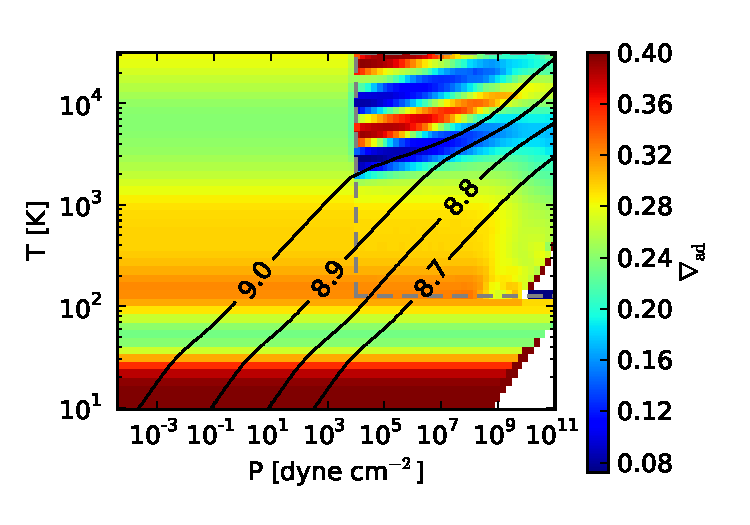
\includegraphics[width=0.5\textwidth]{../../figs/ModelAtmospheres/RadSelfGravRealEOS/PaperFigs/delad_S_mixt.pdf}
%%\vspace{-0.5in}
\caption{Contour plot of the adiabatic gradient $\delad$ for a hydrogen-helium mixture as a function of gas temperature and pressure. The upper-right rectangle encloses the region described by the original \citet{saumon95} EOS tables, while the rest of the plot is our extension. The black curves represent constant entropy adiabats, with the labels $\log_{10}(S)$ [erg K$^{-1}$ g$^{-1}$]. The regions in which the EOS is either invalid or not computed are masked in white. Our extension is only valid for $T \lesssim 2000$ K, since it does not take into account hydrogen dissociation. We choose $T=1500$ K as a conservative temperature cutoff. \citet{saumon95} do not compute the EOS at very high pressures, since hydrogen is solid or may form a Coulomb lattice in this regime, and thus their EOS treatment is no longer valid. While the boundaries of the region in which the free-energy EOS treatment fails can be determined from fundamental thermodynamic constraints, such calculations are not the object of this work. Instead, we choose as boundary a constant entropy curve ($\log(S)=8.4$) above the region in which the \citet{saumon95} model fails. The expressions derived in \App{EOStables} are sufficient to give good results for the colored regions of the extended map, which fully cover the temperature and pressures ranges required by our models. {\bf This caption is extremely long.  I would find a way to defer much of this to text.}}
\label{fig:deladmap}
\end{figure}
%but not the white ones. We note, however, that the temperature and pressure ranges required by our models are fully covered by the colored regions, where our expressions are valid

%If follows that the expressions derived in \App{EOStables} cannot be used to extend the original tables in this temperature and pressure regime. 

%At high temperatures, hydrogen dissociates and ionizes, while at low temperatures the rotational states of the hydrogen molecule are only partially excited and it no longer behaves like an ideal diatomic gas.

%In what follows we explain the behavior of the adiabatic gradient in the three temperature regimes separately.

\vspace{0.2in}

\textbf{1. Intermediate T: Ideal Gas}

For $300$ K $\lesssim T \lesssim 2000$ K, the hydrogen molecule is not energetic enough to dissociate and hydrogen behaves as an ideal diatomic gas with constant $\delad$ (Figure \ref{fig:deladmap}). The helium component of the gas causes a slight increase in the adiabatic index: $\delad \approx 0.3$ in this temperature range rather than 2/7 as is the case for a diatomic gas \footnote{Recall $\delad \equiv \frac{\gamma-1}{\gamma}$ for an ideal gas, with $\gamma$ the adiabatic index: $\gamma=7/5$ for a diatomic gas and 5/3 for a monatomic gas.}.

\vspace{0.2in}

\textbf{2. High T: Dissociation and Ionization of Hydrogen.}

At low temperatures, hydrogen exists in molecular form and has a stable configuration. As the temperature becomes higher than $T \sim 2000-3000$ K, the internal energy of the hydrogen molecule becomes large enough to break the covalent bond between the atoms, and hydrogen starts dissociating. At $T \gtrsim 10,000$ K, hydrogen ionizes. In stellar and giant planet interiors there is little overlap between the two processes: hydrogen is almost entirely dissociated into atoms by the time ionization becomes important. 

As displayed in Figure \ref{fig:deladmap}, the adiabatic gradient decreases significantly in regions of partial dissociation and partial ionization. This behavior is different than that of a mixture of molecular and atomic hydrogen, for which $2/7<\delad<2/5$, or a mixture of protons and electrons, for which $\delad=2/5$. For a mixture of ideal gases, the total internal energy is given by the sum of the internal energies of the individual gases. When a gas dissociates, however, part of the internal energy of the system is used to break down molecules, which reduces the amount of energy available to increase the temperature of the system, thus lowering the adiabatic gradient. The energy required to dissociate depends on the dissociation fraction, which can be determined from the Saha equation (see e.g., \citealt{kippenhahn90}). The dissociation fraction only depends on gas temperature and density, and hence only on the EOS. 

An expression for the adiabatic gradient as a function of the dissociation fraction is presented in \App{deladdiss}. As expected, the adiabatic gradient is $\delad=2/7$ for pure molecular hydrogen and $\delad=2/5$ when hydrogen is fully dissociated, but decreases significantly during partial dissociation and is smallest when half of the gas is dissociated. This is consistent with the behavior we see in Figure \ref{fig:deladmap}. 

The ionization of atomic hydrogen is also dictated by the Saha equation, with the dissociation energy replaced by ionization energy, hence the adiabatic gradient behaves analogously, consistent with Fig. \ref{fig:deladmap}.




\vspace{0.2in}

\textbf{3. Low T: Hydrogen Rotation and Spin Isomers}

As a diatomic molecule, hydrogen has five degrees of freedom, three associated with translational motion and two associated with rotation. The excitation temperature for rotation is $\Theta_r \approx 85$ K \citep{kittel}, hence the rotational states are fully excited at room temperature. As the gas temperature becomes comparable to $\Theta_r$, fewer rotational states are excited, and rotation entirely ceases as $T \rightarrow 0$. We note that at temperatures larger than $\gtrsim 6000$ K, vibrational motions also become important. While at $T\lesssim2000$ K, where our extension of the \citet{saumon95} EOS tables is valid, vibrational motion is negligible, we include these effects in our extension of the EOS for completion (see \App{EOStables} for details).

 Molecular hydrogen occurs in two isomeric forms, parahydrogen and orthohydrogen. Parahydrogen has antiparallel proton spins and thus an antisymmetric wave function. From the Pauli exclusion principle it follows that it can only occupy symmetric rotational states with even angular quantum number $j$ \citep{farkas35}. In contrast, orthohydrogen has parallel proton spins and a symmetric wave function, and can therefore only occupy states with odd $j$. At equilibrium, the relative abundance of the ortho- and para- states is given by the ratio of their partition functions, described in \App{EOStables}. At $T \rightarrow 0$ all hydrogen molecules are in the ground state with $j=0$, which corresponds to parahydrogen.  As the temperature increases, parahydrogen starts converting into orthohydrogen, resulting in an ortho-para equilibrium ratio of 3:1 at room temperature.
 
%During the para-to-ortho conversion, part of the internal energy of the hydrogen molecule is used 

Similarly to the case of dissociation, as $T$ increases, part of the rotational energy $U_{\rm r}$ of the hydrogen molecule is used to convert parahydrogen to orthohydrogen rather than to only increase the temperature, so $U_{\rm r} \propto T$ no longer holds. The adiabatic gradient $\delad$ thus varies with temperature. \App{deladspin} explores the temperature dependence in detail. These $\delad$ variations, which occur for $T \lesssim 300$ K, are displayed in Figure \ref{fig:deladmap}. At higher temperatures, the ortho-para 3:1 equilibrium ratio is reached; no further isomer conversion occurs, and thus $\delad$ remains relatively constant until dissociation temperatures are reached. 



\section{Role of Equation of State}
\label{EOSeffects}

Variations in the adiabatic gradient $\delad$ due to partial dissociation and molecular rotational effects (see \S\ref{deladtable}) affect atmospheric evolution by yielding: (1) a lower envelope luminosity $L$, and (2) a larger amount of radiated energy per unit of accreted mass $-dE/dM$, when compared to an ideal gas. As a result, the rate of change in atmospheric mass,

\begin{equation}
\label{eq:dMdt}
\dot{M} = -\frac{L}{dE/dM},
\end{equation}
(cf. Equation \ref{eq:coolingglobal} and ignoring surface terms) is lower than in the ideal case. The $\delad$ variations thus slow down gas accretion and increase the growth time of the atmosphere, and hence the critical core mass.  

To understand the separate effects of dissociation and rotation on atmospheric growth, we consider the resulting EOS deviations from an ideal gas independently.  
%{\bf In what follows it may be clearer to start with the motivation: isolating the two EOS effects, i.e. dissociation and rotation.  Then introduce the two patched EOSs as how we do this.  Currently it's less clear and more drawn out where this is going.}
In order to explain how quantum rotational states at low temperatures affect atmospheric growth, we 
% {\bf (I don't see how this is a thought experiment, or why we have to imagine.  I would just describe the EOSs)}: 
imagine \textbf{(I used 'imagine' to make it clear that this is just an exercise to isolate the EOS effects, rather than a physically motivated assumption)} that the EOS deviates from a polytrope only in the upper atmosphere where temperatures are low, and that the gas is ideal and polytropic deep in the envelope. Conversely, we study the effects of dissociation at high temperatures by assuming that the EOS is realistic at the bottom of the atmosphere where temperatures are high, but that the gas is polytropic in the outer regions. We compare the behavior of each EOS described above with that of an ideal gas polytrope. Lastly, we use the realistic EOS at all temperatures to study the combined effects of dissociation and rotation. 

%{{\bf Finish the description of the EOSs first.  Then describe and interpret Fig. 2 starting in a new paragraph.  Starting the fig description at the end of a methods discussion lost me.)}  

Figure \ref{fig:tplotall} shows the time evolution of atmospheres forming at 10 AU around cores of mass $M\co=10 M_{\oplus}$ and described by various equations of state, as follows:
%{\bf I would make this list numbered and omit the reference to the curve styles, which is clear in figures.}
\begin{enumerate}
\item Ideal gas polytrope with $\delad=0.3$.
\item Ideal gas polytrope with $\delad=0.3$ for $T>500$ K and realistic EOS for $T<500$ K (hereafter low-$T$ realistic EOS).
\item Ideal gas polytrope with $\delad=0.3$ for $T<500$ and realistic EOS for $T>500$ K  (hereafter high-$T$ realistic EOS).
\item Realistic EOS at all $T$. 
%({\bf Here and elsewhere, I don't like ``fully" realistic, as it implies a perfect EOS.  I would just say realistic at all $T$.})
\end{enumerate}
We choose $T=500$ K as the cutoff temperature because the hydrogen-helium mixture behaves like an ideal gas, with $\delad=0.3$, in this temperature regime (see Figure \ref{fig:deladmap}). 
%{\bf (I find the references to curve numbers distracting in general.  I would try to do less of this and focus on describing the physical effects.  The reader still needs to look at the figure, and there the curves are clearly labelled.)} \sout{As such}, 
%By separately comparing curves (1) and (2), and (1) and (3)  while the difference between curves (1) and (3) accounts for hydrogen dissociation. 
Both dissociation and rotation result in slower cooling for both the high-$T$ and low-$T$ realistic EOSs. 
%decrease the atmospheric accretion rate $\dot{M}$ and thus
%This follows from Equation (\ref{eq:dMdt}), with rotation decreasing $L$ and dissociation increasing $-dE/dM$, as we show further. 
Noting the logarithmic scale in Figure \ref{fig:tplotall}, we see that the combined effect of rotation and dissociation is significantly greater than either individually. %consistent with Equation \ref{eq:dMdt}, since dissociation increases $-dE/dM$ while molecular rotation decreases $L$.
  
 %From Equation \ref{eq:dMdt}, the atmospheric growth time is dependent on 

%The growth time is dependent on both the total energy that must be released (i.e., the rate at which energy is released) and on the luminosity of the atmosphere. {\bf `Rate of energy release' and luminosity are the same thing.  You may be calling $dE/dM$ a `rate' which is confusing.  Again, I think if you introduce and physically explain $\dot{M} = -L/(dE/dM)$ at the outset, then the resulting explanations can more compactly and clearly refer to the terms that matter.}  We explore the \sout{relative} influence of these two factors separately.  {\bf Haven't you already started exploring these factors separately?  Why say this again? Also perhaps worth a note (if not an explanation) that the combined effect is significantly greater than either individually (again noting log scale).}

\begin{figure}[h]
\centering
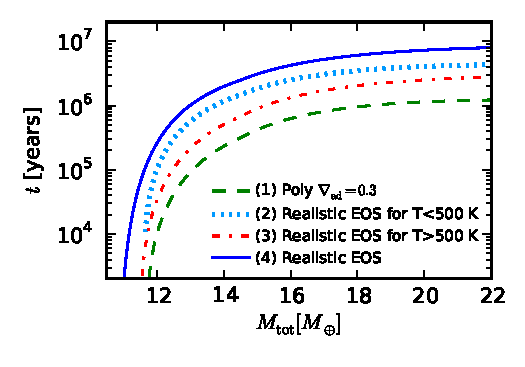
\includegraphics[width=0.5\textwidth]{../../figs/ModelAtmospheres/RadSelfGravRealEOS/PaperFigs/tplot.pdf}
%%\vspace{-0.5in}
\caption{Elapsed time to grow a planet of total mass (core + atmosphere) for a variety of EOS combinations (see text), for a planet forming at 10 AU and with a fixed core mass $M_{\rm c}=10 M_{\oplus}$. Both hydrogen dissociation at high temperatures deep in the atmosphere and molecular rotational effects at low temperatures in the outer envelope result in slower cooling when compared to an ideal gas polytrope.}
\label{fig:tplotall}
\end{figure}

\begin{figure*}[tb]
\centering
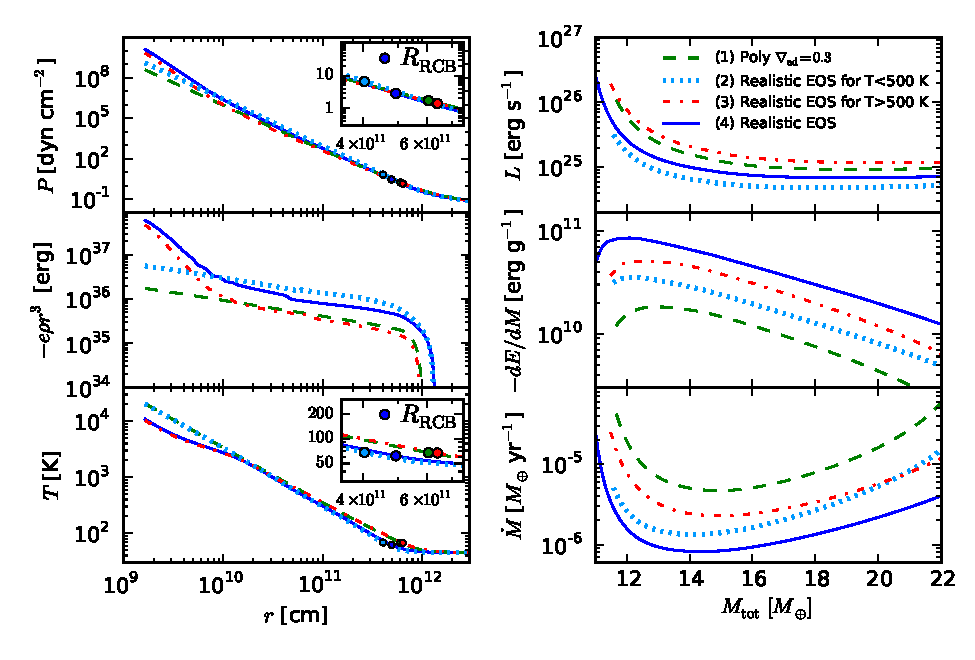
\includegraphics[width=\textwidth]{../../figs/ModelAtmospheres/RadSelfGravRealEOS/PaperFigs/all_plot_test.pdf}
%%\vspace{-0.5in}
\caption{
%{\bf (Left and right panels could be different figs.  The left panel could benefit from showing $P$ or $\rho$.  Also $E_{\rm tot}$ is not yet well defined; the local quantity $e \rho r^3$ might be more instructive.  A greater range of $E$ would show what the polytrope is doing better.  The right panel could benefit from adding $\dot{M}$.  We call $E_{\rm tot} \rightarrow E$ elsewhere, so should be consistent.  Why don't x-axes line up in right panel, are masses different?  What is the discontinuity in $dE/dM$ for the polytrope around 14 $M_\oplus$?  (A kink would be course resolution, but a discontinuity is harder to understand.)  I don't think you need an abs.\ val. around $-dE/dM$.)} 
We explore atmosphere growth around a core of $M\co=10 M_{\oplus}$ forming at 10 AU in our fiducial disk, for the EOS choices in Figure \ref{fig:tplotall}.  Upper-left panel: Radial pressure profile for a total mass (core + atmosphere) of $12 M_{\oplus}$. The location of the RCB is marked. Quantum rotational states at low temperatures in the outer region of the atmosphere result in a deeper RCB. Upper-right panel:  Luminosity evolution as a function of total mass. Rotational effects at low temperatures near the top of the atmosphere result in a lower luminosity for the realistic EOS (see text). Middle-left panel: Total local energy $e \rho r^3$ radial profile for a total mass of $12 M_{\oplus}$. Hydrogen dissociation deep in the atmosphere causes more of the energy to be concentrated at the bottom of the envelope when compared to an ideal gas polytrope. This increases the amount of energy per unit mass that needs to be radiated away, $-dE/dM$.  Middle-right panel:  $-dE/dM$ evolution as a function of total mass. Hydrogen dissociation deep in the atmosphere results in a more negative total energy $E$. Consequently, $-dE/dM$ is larger when compared to the ideal gas polytrope. Lower-left panel:  Radial temperature profile for a total mass of $12 M_{\oplus}$.  Hydrogen dissociation deep in the atmosphere decreases the temperature at the core. This lowers the internal energy and thus results in a more negative total energy $E$.   Lower-right panel: the atmospheric accretion rate $\dot{M}$ as a function of total mass. Both dissociation and rotation reduce $\dot{M}$ and thus slow down atmospheric growth.}
\label{fig:all_plot}
\end{figure*}

The upper-right panel of Figure \ref{fig:all_plot} shows the luminosity evolution with mass for our model EOSs, for a $M\co=10 M_{\oplus}$ core at 10 AU. The realistic EOS effects in the outer envelope decrease the atmospheric luminosity $L$ when compared to an ideal gas polytrope. We can explain this analytically. By substituting Equation (\ref{eq:structa}) into Equation (\ref{eq:structc}) in the convective region of the atmosphere, and assuming the nebular gas obeys the ideal gas law, we can write hydrostatic balance along an adiabat as 

\begin{equation}
\label{eq:dTdr}
\frac{d T}{d r}=-\frac{\delad G m(r)}{\mathcal{R} r^2},
\end{equation}
where $\mathcal{R}$ is the specific gas constant. This result is valid for the $\delad=0.3$ polytrope. As the low$-T$ realistic EOS only slightly (see Figure \ref{fig:deladmap}) deviates from an ideal gas in the outermost convective layers, we can assume that the gas described by the low-$T$ EOS can be approximated as ideal throughout the convective interior. The low-$T$ EOS thus also obeys Equation (\ref{eq:dTdr}) with $\delad \approx const.$. We further neglect self-gravity in Equation (\ref{eq:dTdr}) and set $m(r)=M\co$. Integrating Equation (\ref{eq:dTdr}) from the core to the RCB under these assumptions yields
\begin{equation}
\label{eq:dTdrint}
T\cb=T\co - \frac{\delad G M\co}{\mathcal{R}} \Big(\frac{1}{R\co} - \frac{1}{R\cb}\Big).
\end{equation}  
Deep in the convective interior, $T \gg T\cb$ and $r \ll R\cb$. From virial equilibrium, the temperature in the inner atmosphere can thus be expressed as
\begin{equation}
\label{eq:virialT}
T(r) \simeq \frac{\nabla_{\rm ad} G M\co}{\mathcal{R} r}.
\end{equation}
%The temperature scale height deep in the convective interior is $H_T \sim r$, with $dT/dr \sim -T/H_T \sim -T/r$. From Equation (\ref{eq:structc}) it immediately follows that the pressure scale height, for which $dP/dr \sim -P/H_P$, is $H_P \sim r \delad$. Deep in the interior and for $m(r)=M\co$, hydrostatic balance (\ref{eq:structa}) thus becomes

%\begin{equation}
%\label{eq:structint}
%\frac{P}{r \delad} \sim -\frac{G M\co}{r^2}. 
%\end{equation}
%From this and the definition of the isothermal sound speed
%\begin{equation}
%\label{eq:cs}
%c_s^2 = \frac{P}{\rho} =\mathcal{R} T, 
%\end{equation} 
%with both expressions applied at the core where $r=R\co$, $T=T\co$ and $\delad=\nabla_{\rm ad, c}$, we find
Applying equation (\ref{eq:virialT}) at the core, where $T=T\co$, $r=R\co$ and $\delad=\nabla_{\rm ad, c}$, gives
\begin{equation}
\label{eq:Tc}
T\co \simeq \frac{\nabla_{\rm ad, c} G M\co}{\mathcal{R} R\co}.
\end{equation}
As the adiabatic gradient at the core is the same for both the ideal gas polytrope and the low$-T$ realistic EOS, $T\co$ has the same value for both EOSs. This is shown in Figure \ref{fig:all_plot}, lower-left panel. Substituting Equation (\ref{eq:Tc}) into Equation (\ref{eq:dTdrint}) applied at the RCB gives
\begin{equation}
\label{eq:Tcb}
T\cb \simeq \frac{\nabla_{\rm ad, RCB} G M\co}{\mathcal{R} R\cb},
\end{equation}
%We note that the expression above and the definition of the pressure scale height $H_P \equiv c_s^2 r^2/(G M\co)$ imply that the pressure scale height at the RCB is the same as in the deep interior, $H_P \sim \delad r$.
and thus
\begin{equation}
\label{eq:rcb}
R\cb \propto \frac{\nabla_{\rm ad, RCB}}{T\cb}.
\end{equation}
An approximate expression for $T\cb$ as a function of the adiabatic gradient and disk temperature can be derived using Equation (\ref{eq:delrad}) applied at the RCB (where $\delad=\delrad$) and $\delrad=d \ln T/ d \ln P$ (see Paper I for details). For $\beta=2$ in the opacity law (\ref{eq:opacitylaw}), $T\cb \simeq T\di (1- 2 \nabla_{\rm ad, RCB})^{-1/2}$, and thus
\begin{equation}
\label{eq:rcbdel}
R\cb \propto \frac{\nabla_{\rm ad, RCB}}{(1- 2 \nabla_{\rm ad, RCB})^{-1/2}}.
\end{equation}
For the ideal gas polytrope $\nabla_{\rm ad, RCB}=0.3$, and for the low-$T$ realistic EOS $\nabla_{\rm ad, RCB}\approx 0.25$. For these particular choices, Equation (\ref{eq:rcbdel}) yields a smaller $R\cb$ for the low$-T$ realistic EOS. As such, molecular rotation increases the physical extent, and thus the optical depth of the radiative zone.
%Qualitatively, this can be explained through a simple analytic argument: for a non-self-gravitating atmosphere composed of an ideal gas, the temperature profile in convective regions scales as $T(r) \propto \delad/r$ (see Paper I for details; it can also be derived from Equations \ref{eq:structa} and \ref{eq:structc} applied in convective regions). Applying the expression above at the RCB yields $T\cb \propto \delad\cb/ R\cb$. As the outer radiative layer of the atmosphere is nearly isothermal, $T\cb \approx T\di=const.$, to order unity corrections. It easily follows that $R\cb \propto \deladcb$   Figure \ref{fig:all_plot_temp}, middle-left panel shows 
This is directly correlated to a larger pressure depth of the RCB for the low-$T$ realistic EOS, as shown in the upper-left panel of Figure \ref{fig:all_plot} for a total planet mass of $12 M_{\oplus}$. As $L \propto 1/P\cb$ (cf. Equation \ref{eq:delrad}), the deeper RCB results in a lower $L$ and thus $\dot{M}$ (Figure \ref{fig:all_plot}, lower-right panel).

%directly correlated to the depth of the radiative region of the envelope, which is shown in the upper-left panel of Figure \ref{fig:all_plot} for a total planet mass of $12 M_{\oplus}$. We see that the realistic EOS for low temperatures (2) results in a deeper location of the RCB when compared to the ideal gas polytrope (1). {\bf This is an accurate observation.  
%The deeper question is why does the EOS change result in a deeper RCB?  This should be possible to understand, right?}  This deeper RCB translates into a larger number of steps that photons need to diffuse to escape from the RCB, and therefore a lower luminosity (cf. Equation \ref{eq:delrad}).  {\bf Better to just say it's an optical depth effect than reexplaining how radiative diffusion works.  Also it's the pressure depth (not the radius) that correlates more closely with optical depth.  A plot of $P(r)$ might thus help as noted in fig caption.}

%We see that the lower luminosity of the fully realistic EOS (4) when compared to the polytrope (1) is due to the realistic EOS in the outer atmosphere (2). T

%We found that the RCB for the fully realistic EOS (4) is roughly at the same location as the RCB for the realistic EOS at low temperatures (2) for low atmosphere masses, and it moves further out relatively as the atmosphere mass increases. This explains our choice of $M_{\rm tot}=12 M_{\oplus}$ as a representative case to illustrate the effect of spin isomers. Envelope growth is slowest at this relative atmosphere-to-core mass (see PY13)... 

%Dissociation deep in the planet's atmosphere increases the amount of energy per unit mass that needs to be radiated by the envelope, which further slows down growth. 

%{\bf Why is this true?  Dissociation absorbs energy which by itself decreases the amount of energy that needs to be radiated.}  


Figure \ref{fig:all_plot}, middle-left panel, shows a radial profile of the total local energy $-e \rho r^3$, with $e$ the total specific energy, for the same example planet. \textbf{(the core + total mass choices need to be specified; "the same example planet" is shorter than "for a planet with Mc = ...", and clear enough I think.)}
%the cumulative total energy (internal and gravitational) profile as a function of the radial coordinate, \sout{for the same example planet}. {\bf Two choices: (1) define this cumulative energy more clearly and give it a different symbol than $E_{\rm tot}$ that's already used, maybe $E(r)$, or (2) plot the local (noncumulative) quantity $e \rho r^3$, which should peak in the interesting places.} 
The bulk of the energy is concentrated in the atmospheric interior for all EOSs. However, the energy of the high-$T$ realistic EOS and of the realistic EOS at all $T$ is much larger in magnitude (more negative) near the core when compared to an ideal gas polytrope. This is due to the fact that $\delad$ decreases in dissociation regions (Figure \ref{fig:deladmap}), which results in a shallower temperature gradient and thus lower temperatures near the core. Figure \ref{fig:all_plot}, bottom-left panel shows the radial temperature profile (for $M\co=10 M_{\oplus}$ and $M_{\rm tot}=12 M_{\oplus}$), with temperatures lower near the core for the high-$T$ realistic EOS. As the internal energy $U \propto T$, dissociation decreases $U$ and thus the total energy deep in the interior. This explains the local energy behavior shown in Figure \ref{fig:all_plot}, middle-left panel.  Note that, in some astrophysical contexts, this loss of thermal energy due to dissociation can be so large as to trigger dynamical instabilities and eventual collapse in higher mass objects, such as in protostars \citep{larson69} or during the runaway growth of giant planets \citep{bodenheimer80}.  

The energy behavior can also be explained qualitatively through a simple analytic argument: the density profile in an adiabatic, non-self-gravitating atmosphere composed of an ideal gas scales as $\rho(r) \propto r^{-1/\delad+1}$, and the total specific energy is $e(r) \propto 1/r$ (see Paper I). Thus $e \rho r^3 \sim r^{-1/\delad+3}$. It follows that adiabats with lower $\delad$ have their energy more tightly packed towards the interior of the envelope, which is the case during dissociation. This is consistent with the energy behavior in Figure \ref{fig:all_plot}, middle-left panel. 

We note that the amount of energy that needs to be released in order to accrete gas at the outer boundary is going to be roughly equal for all EOSs, as it has to match the outer boundary conditions of the nebula. However, a more negative total energy in the interior, as is the case for the high-$T$ EOS, requires a larger amount of energy to be radiated away to bind the next batch of gas. This implies a larger $-dE/dM$ during atmospheric evolution (middle-right panel of Figure \ref{fig:all_plot}), and thus a lower $\dot{M}$ for the high-T EOS (lower-right panel of Figure \ref{fig:all_plot}). 

%The high-$T$ realistic EOS has a significantly higher binding energy than the ideal gas polytrope. 

%which increases the amount of energy that needs to be radiated away in order to accrete more gas, i.e. $-dE/dM$. 


 %Dissociation deep in the atmosphere reduces $\delad$, and thus the temperature gradient. Figure \ref{fig:all_plot}, bottom-left panel shows the radial temperature profile (for $M\co=10 M_{\oplus}$ and $M_{\rm tot}=12 M_{\oplus}$). A lower adiabatic gradient results in lower temperatures near the core for the high-$T$ EOS when compared to the ideal gas polytrope. As the internal energy $U \propto T$, dissociation decreases $U$. The total energy $E$ thus becomes more negative

%The bulk of the energy for the high-$T$ realistic EOS and the realistic EOS at all $T$ is , which shows that hydrogen dissociation in the inner atmosphere dictates the energy behavior of the envelope. In contrast, energy is concentrated towards the outer boundary for the $\delad=0.3$ polytrope. 
%{\bf The key question here is how does the slope of the energy affect the quantity that matters, $|dE/dM|$?  This is not clear yet.  I think the shift to lower temperatures, seen in the $T(r)$ plot is helpful, but perhaps the EOS plots should also include an internal energy map.}
%Qualitatively, this can be explained through a simple analytic argument: the density profile in an adiabatic, non-self-gravitating atmosphere composed of an ideal gas scales as $\rho(r) \propto r^{-1/\delad+1}$, and the total specific energy is $e(r) \propto 1/r$ (see Paper I). Thus the total energy scales as $E(r) \propto e(r) \rho(r) r^3 \sim r^{-1/\delad+3}$. It follows that adiabats with lower $\delad$ have their energy more tightly packed towards the interior of the envelope, which is the case during dissociation when $\delad$ decreases significantly (see Section \S\ref{deladtable} and Figure \ref{fig:deladmap}). Dissociation thus causes the atmospheric interior to dominate the total binding energy, which increases the amount of energy that needs to be radiated away in order to accrete more gas, i.e. $-dE/dM$.   

%The larger $-dE/dM$ due to dissociation can also be understood directly from the $\delad$ behavior. Dissociation deep in the atmosphere reduces $\delad$, and thus the temperature gradient. Figure \ref{fig:all_plot}, bottom-left panel shows the radial temperature profile (for $M\co=10 M_{\oplus}$ and $M_{\rm tot}=12 M_{\oplus}$). A lower adiabatic gradient results in lower temperatures near the core for the high-$T$ EOS when compared to the ideal gas polytrope. As the internal energy $U \propto T$, dissociation decreases $U$. The total energy $E$ thus becomes more negative, which translates into a larger $-dE/dM$ during atmospheric evolution (middle-right panel of Figure \ref{fig:all_plot}), and thus a lower $\dot{M}$ for the high-T EOS (lower-right panel of Figure \ref{fig:all_plot}). Note that, in some astrophysical contexts, this loss of thermal energy due to dissociation can be so large as to trigger dynamical instabilities and eventual collapse in higher mass objects, such as in protostars \citep{larson69} or during the runaway growth of giant planets \citep{bodenheimer80}.  

% It takes more energy to bring gas deep into the atmosphere for an envelope that has the bulk of its energy concentrated towards the bottom,  {\bf (This argument isn't clear, new gas isn't brought deep into the atmosphere, it is added at the surface.)} which increases the amount of energy per unit mass that needs to be radiated, i.e. $|dE/dM|$. The cooling time is therefore larger {\bf with dissociation} \sout{for the realistic EOS at high temperatures} (3) when compared to the ideal gas polytrope (1). This increase in $|dE/dM|$ is shown in the bottom-right panel of Figure \ref{fig:all_plot}.

From Equation (\ref{eq:dMdt}), realistic EOS effects reduce the atmosphere accretion rate $\dot{M}$ by decreasing $L$ and increasing $-dE/dM$. This results in slower atmospheric growth and therefore a larger critical core mass, as we show in Section \S\ref{critical}.

%Molecular rotational effects at the top of the atmosphere increase the luminosity $L$, 
%
%We have seen that quantum rotational states transitions due to the low temperatures at the top of the atmosphere {\bf (already too long and convoluted)} increase the thickness of the radiative zone, and decrease the luminosity of the envelope, while dissociation at high temperatures deep in the atmosphere increases the amount of energy needed to increase the atmosphere mass by a fixed amount. {\bf Way too long a sentence!} Overall, both effects result in a longer time for the atmosphere to evolve. 

%we find that only polytropes with $\gamma<3/2$, i.e. $\delad<1/3$, have the total energy concentrated towards the core. This is satisfied by $\delad=2/7$ but not by $\delad=2/5$, in agreement with the results in the bottom panel of Figure \ref{fig:ETrplotpoly}. 
%
%Similarly to section \ref{deladpoly}, we use instantaneous atmosphere profiles to explain the differences. The left panel of Figure \ref{fig:TLrplot} shows the instantaneous temperature profile and the location of the radiative-convective boundary for a total fixed mass (core + atmosphere) $M_{\rm{tot}}=11.8 M_{\oplus}$. The realistic equation of state for low temperatures is characterized by a lower adiabatic index in the outer regions, due to the spin effects, and is therefore dominant in the radiative zone. As a result, it generates a deeper radiative zone with a lower luminosity, which explains the results in the left panel of Figure \ref{fig:TLrplot}. Moreover, since the cooling time is inversely proportional to the luminosity, the spin effect will result in a longer cooling time.
%
%The energy behavior is shown in Figure \ref{fig:Erplot}. The realistic EOS for high temperatures has a low adiabatic index deep in the atmosphere, due to hydrogen dissociation, and thus the bulk of its energy concentrated at the bottom of the atmosphere, for the reasons described in section \ref{deladpoly}. It takes more energy to add mass more mass deep in the atmosphere, and $|dE/dM|$ is larger as a result. 
%%
%
%We have seen that the spin effect at the outer boundary dictates the location of the radiative zone, and therefore the luminosity behavior, while dissociation deep in the atmosphere dictates the energy behavior. Overall, both effects result in a longer time for the atmosphere to evolve. 
%
%\subsection{Ideal Gas Polytropes with Different Adiabatic Gradient}
%\label{deladpoly}
%
%In this section we investigate the differences in luminosity and $dE/dM$, and the resulting time evolution, between ideal gas polytropes with different adiabatic gradients: $\delad=2/7$ (diatomic gas) and $\delad=2/5$ (monatomic gas). We assume both gases have the same mean molecular weight. %We use these results to explain the separate effects of dissociation and spin on the time evolution of the atmosphere.
%
%We generate atmosphere profiles for the two different adiabatic indices at $a=10$ AU and for a core mass $M_{\rm c}=10 M_{\oplus}$, and estimate the luminosity and cooling time evolution as described in section \ref{sec2}. The results are shown in Figure \ref{fig:Ltplotpoly}. We find that the polytrope with the lower adiabatic gradient has both a higher luminosity and a longer cooling time. We use instantaneous atmosphere profiles to explain these effects. 
%
%%We first discuss the effect of the variable adiabatic gradient on luminosity. 
%
%Figure \ref{fig:ETrplotpoly}, top panel, shows the temperature profile for the two polytropes at a fixed total mass $M_{\rm{tot}}=15 M_{\oplus}$. The polytrope with a larger adiabatic gradient, $\delad=2/5$, has a more shallow convective zone, and hence a deeper radiative region, since a larger temperature gradient delays the onset of convection. A deeper radiative layer increases the number of steps that photons need to diffuse, resulting in a lower luminosity as seen in the top panel of Figure \ref{fig:Ltplotpoly}. 
%
%\begin{figure}[h]
%\centering
%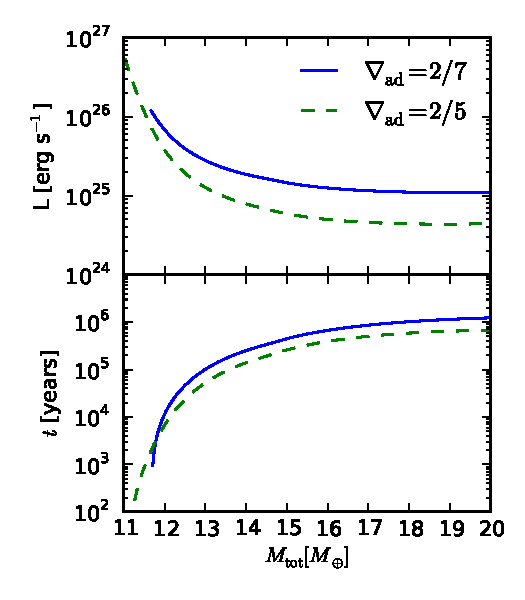
\includegraphics[width=0.5\textwidth]{../../figs/ModelAtmospheres/RadSelfGravRealEOS/PaperFigs/Ltplot_poly.pdf}
%%%\vspace{-0.5in}
%\caption{Luminosity and time evolution as a function of total mass (core + atmosphere) for polytropes with different adiabatic indices, for a planet forming at 10 AU and with a fixed core mass $M_{\rm c}=10 M_{\oplus}$. A larger adiabatic index results in both a lower luminosity and a shorter cooling time.}
%\label{fig:Ltplotpoly}
%\end{figure}
%
%\begin{figure}[h]
%\centering
%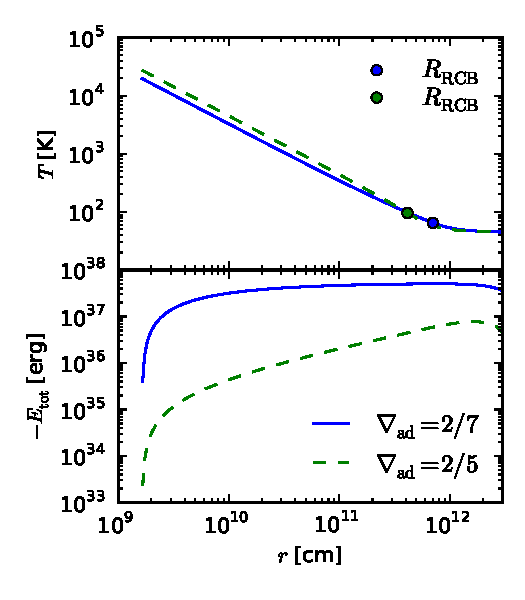
\includegraphics[width=0.5\textwidth]{../../figs/ModelAtmospheres/RadSelfGravRealEOS/PaperFigs/TErplot_poly.pdf}
%%%\vspace{-0.5in}
%\caption{Instantaneous temperature and total energy profiles as a function of radius for polytropes with different adiabatic indices, for a planet forming at 10 AU and with a fixed core mass $M_{\rm c}=10 M_{\oplus}$. The total mass (core + atmosphere) is $15 M_{\oplus}$. The location of the radiative-convective boundary is marked. A lower adiabatic gradient results in a more shallow radiative region (upper panel), and in the total energy being concentrated at the bottom of the atmosphere (lower panel).}
%\label{fig:ETrplotpoly}
%\end{figure}
%
%%In spite of the low luminosity of the atmosphere with $\delad=2/5$, the envelope still grows faster than in the case of a diatomic gas, as shown in the bottom panel of Figure \ref{fig:Ltplotpoly}. This is due to fact that the amount of energy per unit mass that needs to be radiated away, i.e. $|dE/dM|$, is lower for the $\delad=2/5$ polytrope. We have shown in PY13 that polytropes with $\delad=2/7$ have most of the energy concentrated at the bottom of the atmosphere, while polytropes with $\delad=2/5$ have the bulk of the energy towards the outer boundary. 
%
%
%The bottom panel of Figure \ref{fig:ETrplotpoly} shows an instantaneous energy profile for the same total mass $M_{\rm{tot}} = 15 M_{\oplus}$.  The bulk of the energy is concentrated deep in the atmosphere for the $\delad=2/7$ polytrope and towards the outer boundary for the $\delad=2/5$ polytrope. Qualitatively, this can be explained through a simple analytic argument: the density profile in an adiabatic, non-self gravitating atmosphere composed of an ideal gas scales as $\rho(r) \sim r^{1/(\gamma-1)}$ with $\gamma$ the adiabatic index (see PY13). Since the energy per unit mass scales as $e(r) \sim \rho(r) r^2$, we find that only polytropes with $\gamma<3/2$, i.e. $\delad<1/3$, have the total energy concentrated towards the core. This is satisfied by $\delad=2/7$ but not by $\delad=2/5$, in agreement with the results in the bottom panel of Figure \ref{fig:ETrplotpoly}.  It takes more energy to bring in gas deep in the atmosphere for an envelope that has the bulk of its energy concentrated towards the bottom,  which increases $|dE/dM|$ for the $\delad=2/7$ polytrope. 
%
%We find that the energy effect prevails over the luminosity effect, resulting in a longer cooling time for the polytrope with the lower adiabatic gradient (i.e., $\delad=2/7$), as shown in the bottom panel of Figure \ref{fig:Ltplotpoly}.


%From the adiabatic gradient table shown in Figure \ref{fig:deladmap} we find that $\delad$ has the flattest behavior around $T=500$ K. In this region, the gas behaves like an ideal gas with constant polytropic index $\delad \approx 0.3$, with the shift from diatomic gas caused by the helium in the mixture. We generate three sets of atmosphere profiles. The first one corresponds to an ideal gas of constant adiabatic index $\delad=0.3$. The second one is described by the real EOS for temperatures larger than 500 K and by an ideal gas with $\delad=0.3$ for $T<500$ K. Finally, the third profile consists of an ideal gas polytrope with $\delad=0.3$ for $T>500$ K and a real gas in the low temperature regime. We compare the first two profiles to show the dissociation effects, and the first and third profile to show the effects of ortho- and parahydrogen. The resulting time evolution is shown in Figure \ref{fig:Ltplotall}. We see that both dissociation and spin isomers have a comparable effect on the atmosphere growth, and result in slower cooling, and therefore a longer crossover time, when compared to the polytropic ideal gas equation of state. In what follows we explore the two effects separately.




%As compared to the polytrope, the real EOS therefore generates a deeper radiative zone with a lower luminosity, due to the lower adiabatic index in the outer regions, as well as an atmosphere with the bulk of its energy concentrated at the bottom, due to the low $\delad$ caused by dissociation. As shown above for the ideal gas polytropes, and remembering that $\Delta t \sim -\Delta E/L$, we see that both effects result in a longer time for the atmosphere to evolve.  


 



% for an atmosphere described by an ideal gas EOS with $\delad=0.3$ (dashed curve), an atmosphere composed of an ideal gas with $\delad=0.3$ for $T>500$ K and a realistic gas 

%In this section we use the results obtained in section \ref{deladpoly} to explain the effects on the atmosphere evolution of a realistic equation of state. We explore the effect of hydrogen dissociation at the high temperatures in the inner part of the atmosphere, and the effect of hydrogen spin isomers at the low temperatures at the top of the atmosphere separately. In order to do this, we generate atmosphere profiles in which the nebular gas is assumed to be described by a combination of ideal and realistic equations of state, depending on the temperature. To explain the effects of the hydrogen spin isomers in the outer parts of the atmosphere, we assume that the realistic EOS effects only matter at low temperatures; conversely, we assume that the realistic EOS effects are important only at high temperatures in order to study the effects of hydrogen dissociation deep in the atmosphere. As such, we generate three sets of atmosphere profiles, choosing $a=10$ AU and $M\co=5 M_{\oplus}$. The first one is described by a realistic EOS for temperatures larger than 500 K and by an ideal gas with $\delad=0.3$ for $T<500$ K. The second profile consists of an ideal gas polytrope with $\delad=0.3$ for $T>500$ K and a realistic gas in the low temperature regime. Finally, the last profile corresponds to an ideal gas with $\delad=0.3$, the adiabatic gradient of an ideal hydrogen-helium mixture.  We choose $T=500$ K as the reference temperature since the adiabatic gradient of the realistic gas is roughly constant around this temperature (see Figure \ref{fig:deladmap}). The differences in atmosphere structure and evolution between the ideal gas and the realistic gas at low (high) temperatures highlight the effects of hydrogen spin isomers (hydrogen dissociation). Figure \ref{fig:tplotall} illustrates the differences in time evolution between these profiles. We see that both dissociation and spin isomers have a comparable effect on the atmosphere growth, and result in slower cooling, and therefore a longer crossover time, when compared to the polytropic ideal gas equation of state. The cooling time is dependent on both the total energy released due to the contraction of the envelope and the luminosity of the atmosphere. In what follows we explore the relative influence of these two factors separately.


%The resulting time evolution is shown in Figure \ref{fig:tplotall}. We see that both dissociation and spin isomers have a comparable effect on the atmosphere growth, and result in slower cooling, and therefore a longer crossover time, when compared to the polytropic ideal gas equation of state. The cooling time is dependent on both the total energy released due to the contraction of the envelope and the luminosity of the atmosphere. In what follows we explore the relative influence of these two factors separately.

%We now discuss the differences in luminosity and $dE/dM$ between an ideal gas with constant adiabatic gradient and atmospheres with variations in $\delad$ as prescribed by the equation of state discussed in section \ref{EOSeffects}. In what follows we describe our choices of equation of state combinations. From the adiabatic gradient table shown in Figure \ref{fig:deladmap} we find that $\delad$ has the flattest behavior around $T=500$ K. In this region, the gas behaves like an ideal gas with constant polytropic index $\delad \approx 0.3$, with the shift from diatomic gas caused by the helium in the mixture. We generate three sets of atmosphere profiles. The first one corresponds to an ideal gas of constant adiabatic index $\delad=0.3$. The second one is described by the realistic EOS for temperatures larger than 500 K and by an ideal gas with $\delad=0.3$ for $T<500$ K. Finally, the third profile consists of an ideal gas polytrope with $\delad=0.3$ for $T>500$ K and a realistic gas in the low temperature regime. We compare the first two profiles to show the dissociation effects, and the first and third profile to show the effects of ortho- and parahydrogen. The resulting time evolution is shown in Figure \ref{fig:tplotall}. We see that both dissociation and spin isomers have a comparable effect on the atmosphere growth, and result in slower cooling, and therefore a longer crossover time, when compared to the polytropic ideal gas equation of state. The cooling time is dependent on both the total energy released due to the contraction of the envelope and the luminosity of the atmosphere. In what follows we explore the relative influence of these two factors separately.

%We now investigate the effect of the low adiabatic index caused by hydrogen dissociation, on the one hand, and spin isomers on the other hand, on the luminosity and cooling time evolution of the atmosphere, in light of the discussion in section \ref{deladpoly}. The left panel of Figure (x) shows the luminosity evolution with mass for the four combinations of equations of state described in section  

%
%
%\begin{figure}[h]
%\centering
%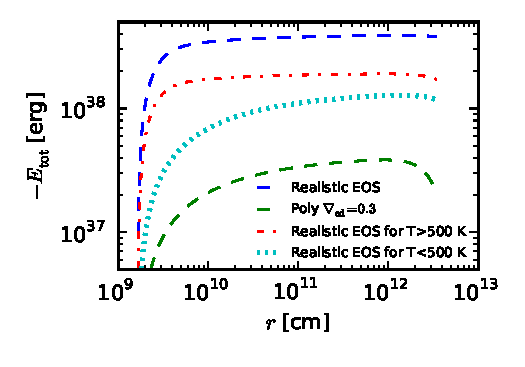
\includegraphics[width=0.5\textwidth]{../../figs/ModelAtmospheres/RadSelfGravRealEOS/PaperFigs/Er_plot.pdf}
%%%\vspace{-0.5in}
%\caption{Instantaneous energy profiles as a function on radius for a variety of EOS combinations, for a planet forming at 10 AU and with a fixed core mass $M_{\rm c}=10 M_{\oplus}$. The total mass (core + atmosphere) is $11.8 M_{\oplus}$. Hydrogen dissociation deep in the atmospheres causes the bulk of the energy to be concentrated at the bottom of the atmosphere. This increases the amount of energy per unit mass that needs to be radiated away, i.e. $|dE/dM|$, resulting in a longer crossover time for the realistic EOS when compared to the polytrope.}
%\label{fig:Erplot}
%\end{figure}


\section{Opacity Effects on Atmosphere Evolution}
\label{sec:opacity}


So far in our model we have assumed that the dust opacity in the radiative region of the atmosphere is given by the standard ISM opacity. However, our scenario of low planetesimal accretion is likely to favor lower dust opacities, due to grain growth and dust settling. Grain growth, in particular, changes the particle size distribution when compared to the standard ISM size distribution (e.g., \citealt{pollack85}) and lowers the absolute value of the opacity. Enhanced metallicity due to planetesimal accretion, by construction not present during our atmosphere's growth, cannot make up for this reduction.

%Observations of dust in protoplanetary disks (e.g., \citealt{beckwith90}, \citealt{beckwith91}, \citealt{perez12}) have shown evidence for grain growth and that the particle size distribution is not interstellar. 

Although grain growth and evidence for a non-ISM size distribution have been observed in protoplanetary disks (e.g., \citealt{beckwith90}, \citealt{beckwith91}, \citealt{perez12}), the size distribution of dust particles has not been tightly constrained. Typically, the grain size distribution is assumed to be a power-law: 

\begin{equation}
\label{eq:graindistr}
n(a) \sim a^{-p},
\end{equation}
where $n(a)$ is the number density of particles of size $a$ and $p=3.5$ (corresponding to a ``normal'' collisional cascade) or $p=2.5$ (an approximation for coagulation). In this work we use the  \citet{dalessio01} frequency-dependent opacity tables to obtain the temperature-dependent Rosseland mean opacity $\kappa$. We take as a fiducial case a maximum particle size of 1 cm and a grain size distribution given by Equation (\ref{eq:graindistr}) with $p=3.5$. Other choices for the power-law coefficient $p$ are discussed later in this section. 

The \citet{dalessio01} opacities are only relevant at temperatures that are sufficiently low for dust grains to remain solid ($T \lesssim 1000$ K). In the temperature regime where dust sublimates we use the \citet{bell94} analytic opacity laws, ensuring smooth transition from the grain growth opacities. 

The sharp drop in opacity ($\kappa \sim T^{-24}$, see Figure \ref{fig:delvsr}) due to dust sublimation lowers the radiative temperature gradient significantly (see Equation \ref{eq:delrad}), and may therefore generate radiative layers within the inner region of the atmosphere (see \App{radwindow}, Figure \ref{fig:delvsr}). This could in principle pose challenges for our model, since the additional luminosity generated in these radiative windows may be large enough to make our assumption of constant luminosity throughout the radiative layers invalid. In practice, however, the inner radiative windows are either very thin (Figure \ref{fig:delvsr}, middle panel), or the temperature gradient is flat enough to result in a roughly constant luminosity throughout the region (Figure \ref{fig:delvsr}, bottom panel; also see Equation \ref{eq:structc}). This results in a negligible extra luminosity generated in the radiative windows. However, the radiative windows may become non-negligible for other opacity choices and sufficiently low core masses, as we show later in this section. We note that despite the existence of one or more radiative windows in the planet's atmosphere, the luminosity that emerges at the outer boundary is set by the outer radiative layer. In fact, a simple estimate of the luminosity emerging at the RCB can be found as follows. 

The equation of radiative diffusion (\ref{eq:structc}) can be approximated in terms of the radiative flux $\mathcal{F}$ as 

\begin{equation}
\label{eq:sigmatau4}
\mathcal{F} \sim \frac{\sigma T\cb^4}{\tau},
\end{equation}
where $\tau$ is the optical depth of the upper radiative layer. Furthermore, we find that $\tau$ is dominated by the optical depth of the first scale height, i.e. 

\begin{equation}
\label{eq:taucb}
\tau \sim \tau\cb=\kappa\cb \rho\cb H\cb,
\end{equation}
with
\begin{equation}
\label{eq:Hcb}
H\cb=\frac{k_B T\cb}{\mu m_p} \frac{R\cb^2}{G M\cb},
\end{equation}
where $\mu$ is the mean molecular weight of the gas, $m_p$ the proton mass, and all other quantities are evaluated at the RCB. By substituting Equations (\ref{eq:Hcb}) and (\ref{eq:taucb}) into Equation (\ref{eq:sigmatau4}), and noting that $\mathcal{F}=L/(4 \pi (R\cb+H\cb)^2) \approx L / (4 \pi R\cb^2)$, we recover Equation (\ref{eq:delrad}) applied at the boundary between the uppermost convective region of the atmosphere and the outer radiative layer (where $\delrad=\delad$) as

\begin{equation}
\label{eq:Lapprox}
L \sim \frac{4 \pi \sigma T\cb^3 G M\cb \mu m_p}{k_B \kappa\cb \rho\cb}.
\end{equation}
Equation (\ref{eq:Lapprox}) can be used to estimate the luminosity emerging at the top of the convective layer of the atmosphere. We have verified that the luminosity emerging at the bottom of the outer radiative layer in our models can indeed be approximated by Equation (\ref{eq:Lapprox}). %As $T\cb$ only differs from the disk temperature by an order unity factor, $L\sim 1/\rho\cb$. The change in EOS thus results in a deeper RCB and a lower luminosity.  

Due to the variable number and position of radiative windows, and therefore radiative-convective boundaries, within the planet atmosphere, we cannot consistently calculate the time evolution of different atmospheres if we evaluate our cooling Equation (\ref{eq:coolingglobal}) at the RCB, as we do in our standard model. We choose to evaluate the cooling time at the Bondi radius instead (since our cooling model applies at any radius $R$, see section \S\ref{struct}). We note that our choice of $R$ does not change the estimate of the atmosphere evolution time, to order of magnitude, since the additional luminosity generated in all radiative regions is negligible for our opacity choice (also see Paper I). 




%\subsection{Outer Boundary Effects}

%\textbf{Reemphasize the fact that the atmosphere structure is determined by your outer boundary conditions: T_{out}, P_{out}, R_{out} $\rightarrow$ explore the separate effects of pressure, temperature and a (since the Hill radius is determined by a); show how temperature is the strongest effect. }

\section{Critical Core Mass}
\label{critical}

%\textbf{Define what it is (refer again to paper I also); show the Mcrit vs a for fixed disk life plot, for both real EOS, gamma 7/5 and gamma 5/3; justify the differences in terms of the EOS effects from 4.2; show that using a real EOS makes a significant difference to the results; however, the core masses we get are still doable. Again, a lot of text below will be used but needs reorganizing/rephrasing.}

%\textbf{Define what it is (also refer to paper I) and emphasize how it's different from $M_{crit}$ in standard calculations. Define the crossover mass and crossover time.}


In this section we put together the results obtained in Sections \S\ref{EOSeffects}  and \S\ref{sec:opacity}, and determine the minimum core mass to initiate runaway gas accretion during the lifetime of the protoplanetary disk, i.e. the critical core mass. As in Paper I, we quantify the runaway growth timescale $t_{\rm run}$ as the time at which the atmosphere growth time $M_{\rm atm}/\dot{M}$ drops to 10\% of its maximum value (see Paper I for details). We first explore the dependence of the runaway growth time on the core mass for a fixed semimajor axis. We then determine the critical core mass to form a giant planet from a gas composed of a realistic hydrogen-helium mixture, and we compare this with the results from Paper I for an ideal diatomic gas. Finally, we determine the critical core mass under more realistic opacity assumptions.

%\subsection{Crossover Time as a Function of Core Mass}
%\label{tvsM}

%\textbf{t vs. M at fixed distance, similar to the plot from paper I. Compare scalings.}

Figure \ref{fig:tvsMplot} displays the time evolution and the runaway growth time for atmospheres forming around cores with masses between 10 $M_{\oplus}$ and 20 $M_{\oplus}$ at $a=10$ AU in our fiducial disk. Higher mass cores have both shorter $t_{\rm run}$ and fractionally larger atmosphere masses at runaway, consistent with the results of Paper I. 

\begin{figure}[h!]
\centering
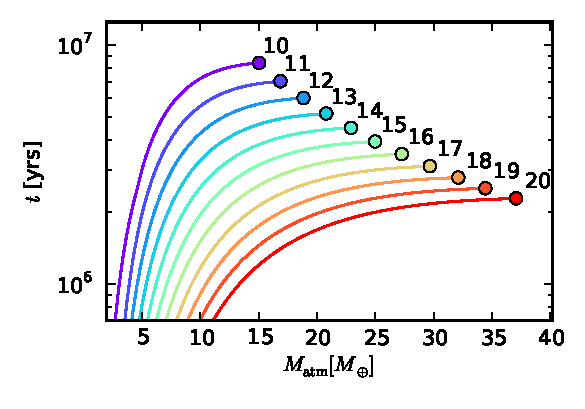
\includegraphics[width=0.5\textwidth]{../../figs/ModelAtmospheres/RadSelfGravRealEOS/PaperFigs/t_vs_M_10au.pdf}
%%\vspace{-0.5in}
\caption{Elapsed time as a function of atmosphere mass, for cores with fixed masses between $10 M_{\oplus}$ and $20 M_{\oplus}$ at $a=10$ AU in our fiducial disk. The circles mark the runaway growth time. The numbers are labeling the core mass in Earth masses. A larger core mass results in a lower $t_{\rm run}$ and a higher $M_{\rm atm}/M\co$ at runaway.}
\label{fig:tvsMplot}
\end{figure}

%\subsection{Critical Core Mass}
%\label{Mcrit}

%\textbf{Mcrit vs. a plot, realistic EOS and polytrope. Discuss the larger critical core mass for the real EOS in light of the effects from section 4.}

Figure \ref{fig:Mvsaplot} shows the critical core mass for a massive atmosphere to form during a typical lifetime of a protoplanetary disk $t=3$ Myrs (e.g., \citealt{jay99}), for a gas described by a realistic EOS and an ISM dust opacity given by Equation (\ref{eq:opacitylaw}) with $F_{\kappa}=1$ and $\beta=2$. The results of Paper I for an ideal diatomic gas are plotted for comparison. The use of a realistic EOS results in a critical core mass more than twice as large as that produced by a polytrope. As such, non-ideal effects substantially increase the core mass needed to form a giant planet  before the dissipation of the protoplanetary disk.   

\begin{figure}[h!]
\centering
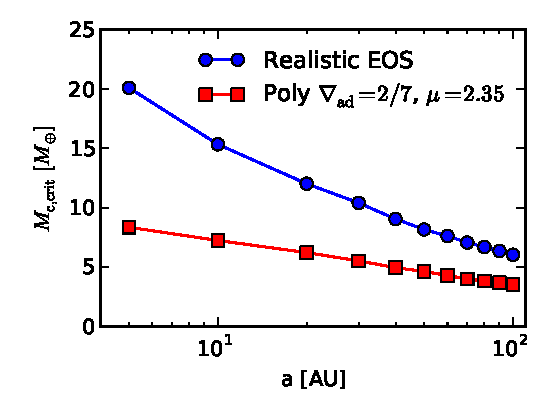
\includegraphics[width=0.5\textwidth]{../../figs/ModelAtmospheres/RadSelfGravRealEOS/PaperFigs/Mc_vs_a_poly_real_paper.pdf}
%%\vspace{-0.5in}
\caption{The minimum core mass for an atmosphere to initiate runaway gas accretion within the lifetime of a typical protoplanetary disk $t \sim 3$ Myrs as a function of semimajor axis, for a realistic hydrogen-helium mixture and a standard ISM power-law opacity. The results of Paper I for an ideal diatomic gas are plotted for comparison. The realistic EOS yields core masses larger by more than a factor of 2 when compared to the polytrope.}
\label{fig:Mvsaplot}
\end{figure}


\begin{figure}[h!]
\centering
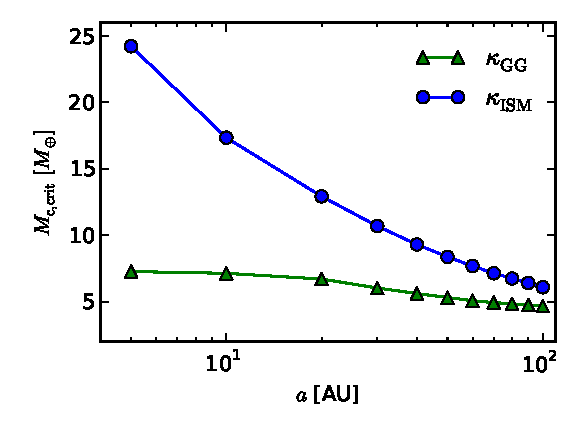
\includegraphics[width=0.5\textwidth]{../../figs/ModelAtmospheres/RadSelfGravRealEOS/PaperFigs/Mcrit_vs_a_gg.pdf}
%%\vspace{-0.5in}
\caption{Critical core mass as a function of semimajor axis for radiative opacities that account for grain growth (green triangles, with $p=3.5$ and $a_{\rm max}=1$ cm; see text for details). The critical core mass is lower than it would be if dust grains had an ISM-like size distribution (blue circles).}
\label{fig:Mcritvsagg}
\end{figure}

Figure \ref{fig:Mcritvsagg} shows the critical core mass as a function of semimajor axis, for a grain growth opacity with a size distribution given by the power-law (\ref{eq:graindistr}) with $p=3.5$ and maximum particle size of 1 cm. The critical core mass is lower than in the standard case, and less sensitive to location in the disk, i.e. the boundary conditions (temperature and pressure). We have shown in Paper I that the critical core mass is highly dependent on disk temperature rather than pressure. The temperature dependence, however, is mainly due to opacity. For the simplified analytic model developed in Paper I we found that the crossover time $t_{\rm co} \sim T_{\rm d}^{\beta+1/2}$, with $\beta$ the power-law exponent in Equation (\ref{eq:opacitylaw}) and $t_{\rm co}$ a proxy for $t_{\rm run}$, defined as the time when $M_{\rm atm}=M\co$, as $t_{\rm run}$ cannot be determined self-consistently for the analytic model. Opacity is less sensitive to temperature variations for larger grains and has an almost flat profile (see Figure \ref{fig:opacity}), which results in $\beta \ll 1$ and a much weaker temperature (and therefore semimajor axis) dependence of the critical core mass, as seen in Figure \ref{fig:Mcritvsagg}. Moreover, grain growth reduces the absolute value of the opacity, which results in an overall lower runaway accretion time and critical core mass. % As noted in Section \S\ref{sec:opacity}, the critical core mass may be significantly lower if coagulation is taken into account, i.e. $p=2.5$.

\begin{figure}[h!]
\centering
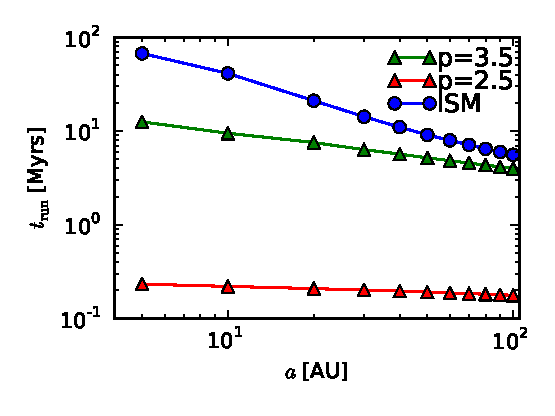
\includegraphics[width=0.5\textwidth]{../../figs/ModelAtmospheres/RadSelfGravRealEOS/PaperFigs/tco_vs_a_Mc4_comp.pdf}
%%\vspace{-0.5in}
\caption{Runaway accretion times for different grain size distributions, for an atmosphere forming around a core with $M\co=4 M_{\oplus}$. The lines marked by green and red triangles have grain growth opacities with $a_{\rm max}=1$ cm, and $p=3.5$ and $p=2.5$, respectively (see text for details). The blue circle line has an ISM power-law opacity. The runaway accretion time is more than one order of magnitude lower when coagulation is accounted for, i.e. $p=2.5$.}
\label{fig:p25p35}
\end{figure}

So far we have assumed that the size distribution of dust grains is a power-law (\ref{eq:graindistr}) with $p=3.5$ which corresponds to a normal collisional cascade. If, however, coagulation is taken into account, the exponent $p$ can be approximated as $p=2.5$ \citep{dalessio01}. This results in a flatter and significantly lower opacity, which may substantially reduce the critical core mass. However, we have found that our model breaks down for low core masses ($M\co \lesssim 3 M_{\oplus}$) under our assumption of constant luminosity in the outer radiative layer. Figure \ref{fig:p25p35} shows the crossover time $t_{\rm co}$ as a function of semimajor axis for the lowest core mass for which our model is valid, $M\co=4 M_{\oplus}$. The crossover time is more than one order of magnitude lower for $p=2.5$, which implies that the critical core mass may be, in fact, significantly lower than presented in Figure \ref{fig:Mcritvsagg}.

%Figure \ref{fig:p25p35} shows the crossover time $t_{\rm co}$ as a function of semimajor axis for a core of mass $M\co=4 M_{\oplus}$ and for two choices of the exponent $p$ in the power-law (\ref{eq:graindistr}): $p=3.5$, which corresponds to a normal collisional cascade, and $p=2.5$, which accounts for coagulation \citep{dalessio01}. We choose $M\co=4 M_{\oplus}$ as our model breaks down for lower core masses ($M\co \lesssim 3 M_{\oplus}$) under our assumption of constant luminosity in the outer radiative layer. The crossover time is lower for both choices of $p$ when compared to $t_{\rm co}$ when an ISM opacity is assumed. Moreover, $t_{\rm co}$ is more than one order of magnitude lower for $p=2.5$ than for $p=3.5$. As $t_{\rm co}$ is lower than the typical disk lifetime of a few Myrs for $M\co=4 M_{\oplus}$ and $p=2.5$, the critical core mass under these assumptions is lower than the core mass for which our model is valid. We thus cannot accurately calculate $M_{\rm crit}$ for $p=2.5$ and choose $p=3.5$ as our fiducial case. We note, however, that the critical core mass may be, in fact, significantly lower that the results we present in \S\ref{critical}.



%So far we have assumed that the size distribution of dust grains is a power-law (\ref{eq:graindistr}) with $p=3.5$, which corresponds to a normal collisional cascade. If, however, coagulation is taken into account, the exponent $p$ can be approximated as $p=2.5$ \citep{dalessio01}. This results in a flatter and significantly lower opacity, which may substantially reduce the critical core mass. However, we have found that our model breaks down for low core masses ($M_{\rm c} \lesssim 3 M_{\oplus}$) under this assumption, i.e. the outer radiative zone becomes deep enough that the luminosity generated in this region can no longer be neglected. The crossover time is more than one order of magnitude lower for $p=2.5$, which implies that the critical core mass may be, in fact, significantly lower than presented in Figure \ref{fig:Mcritvsagg}. 



%\section{Model Relevance in Planet Formation Theory}
\section{Effects of Planetesimal Accretion}
\label{acc}

In this study we have considered protoplanets with fully formed cores for which planetesimal accretion is negligible and KH contraction dominates the luminosity evolution of the atmosphere. This is different from calculations that assume high planetesimal accretion rates and find that the atmosphere is in steady state and solely heated due to accretion of solids. In this section we compare our results for the critical core mass to analogous results from steady-state fast planetesimal accretion calculations. We discuss the core accretion rates that are necessary for our regime to be valid in \S\ref{raf1}. In \S\ref{raf3}, we estimate core growth during atmosphere evolution at the maximum rate for which the KH regime is valid, and show it is negligible. Finally, we compare our results with those assuming fast planetesimal accretion in \S\ref{raf2}.

 %In this section we investigate the core accretion rates that are necessary for our regime to be valid. We also discuss the conditions under which runaway gas accretion can be initiated due to the Kelvin-Helmholtz contraction of the atmosphere before it becomes critical due to planetesimal accretion.

\subsection{Planetesimal Accretion Rates}
\label{raf1}

Kelvin-Helmholtz contraction dominates an atmosphere's luminosity if  $L_{\mathrm{acc}} < L_{\rm{KH}}$, where $L_{\rm{acc}}$ is the accretion luminosity,

\begin{equation}
\label{eq:Lacc}
L_{acc}=G \frac{M_{\rm{c}} \dot{M_{\rm{c}}}}{R_{\rm{c}}},
\end{equation}
and $L_{\rm KH}$ is given by Equation (\ref{eq:coolingglobal}) with $L\co=\Gamma=0$. This condition is satisfied as long as the planetesimal accretion rate 

\begin{equation}
\label{eq:McdotKH}
\dot{M\co}<\dot{M}_{\rm c, KH} \equiv \frac{L_{\rm KH} R\co}{G M\co}.
\end{equation} 

To illustrate the magnitude of $\dot{M}_{\rm c, KH}$, we choose as a fiducial case an atmosphere forming at 10 AU and with a core mass of $10 M_{\oplus}$. Since analytic studies of critical core masses at high planetesimal accretion rates assume an ideal gas EOS, for ease of comparison we choose an ideal gas polytrope with constant adiabatic gradient $\delad=2/7$ and mean molecular weight $\mu=2.35$ (see also Paper I). For this choice of parameters, the runaway accretion time is $t _{\rm run}\sim$ 1.3 Myrs, which is within the typical lifetime of a protoplanetary disk. We also estimate two reference accretion rates. The first one is the core accretion rate $\dot{M}_{\rm c, acc}$ needed to grow the core to $M\co=10 M_{\oplus}$ on the same timescale as our model atmosphere, $\tau=1.3$ Myrs:

\begin{equation}
\label{eq:Mcdot}
\dot{M}_{\rm{c,acc}}(M_{\rm{c}}) \equiv \frac{M_{\rm{c}}}{\tau}.
\end{equation}
The second reference planetesimal accretion rate is $\dot{M}_{\rm c, Hill}$, a typically assumed planetesimal accretion rate for which the random velocities of the planetesimals are of the order of the Hill velocity around the protoplanetary core (for a review, see \citealt{goldreich04}). Following R06 (equation A1),

%This is the accretion rate at the boundary between the dispersion dominated and shear dominated regimes. 

\begin{equation}
\label{eq:MdotHill}
\dot{M}_{\rm{c,Hill}}=\Omega \Sigma_{\rm p} R\co R_{\rm H},
\end{equation}
where $\Sigma_{\rm p}$ is the surface density of solids, assumed to satisfy $\Sigma\di \approx 100 \Sigma_{\rm p}$ for a dust-to-gas ratio of 0.01.

Figure \ref{fig:accrates} shows that $\dot{M}_{\rm c,KH}$ is $\sim2-3$ orders of magnitude lower than $\dot{M}_{\rm c, acc}$. Had the core accreted planetesimals at the $\dot{M}_{\rm c, KH}$ rate since it started forming, it could not have grown large enough to attract an atmosphere within typical disk lifetime. This is consistent with the results of \citet{pollack96}, which find that the planetesimal accretion rate decreases with time as the core's feeding zone is depleted, and with the requirement of our model that the planetesimal accretion rate is initially large during core growth, then significantly reduces as the gaseous envelope accumulates. This is a plausible scenario, as the core may have formed in the inner part of the disk and was later scattered outwards \citep{ida13}, or the planet's feeding zone could have been depleted of solids due to a giant neighbor.  


 \begin{figure}[h]
\centering
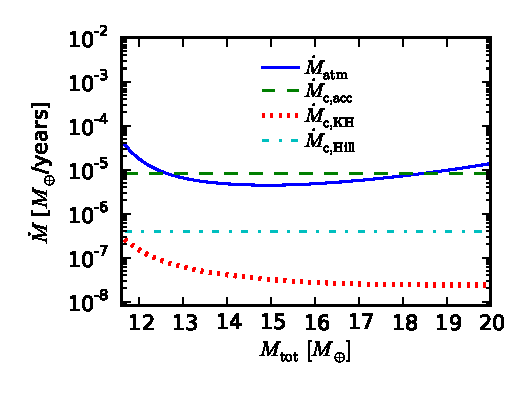
\includegraphics[width=0.5\textwidth]{../../figs/ModelAtmospheres/RadSelfGravRealEOS/PaperFigs/acc_rates_paper.pdf}
%\vspace{-0.5in}
\caption{Various accretion rates for a planet forming at 10 AU and with a core mass $M\co=10 M_{\oplus}$, using a polyropic EOS and ISM power-law opacity. For this choice of parameters, the runaway accretion time is $t_{\rm run} \sim 1.3$ Myrs. The $\dot{M}_{\rm{atm}}$ (solid blue) curve represents the growth rate of the atmosphere as estimated by our model. The core accretion rate $\dot{M}_{\rm c, acc}$ (dashed green) necessary to grow the core on the timescale $t_{\rm run}$ is larger than $\dot{M}_{\rm c, KH}$ (dotted red), the maximum planetesimal accretion rate during KH contraction for which our regime is valid (see text). The $\dot{M}_{\rm c, acc}$ rate is also larger than the frequently used planetesimal accretion rate $\dot{M}_{\rm c, Hill}$ (dashed-dotted light blue) for which the random velocity of the planetesimals is given by the Hill velocity due to the core (see text). 
This motivates our requirement  that planetesimal accretion must have slowed down after core growth for our model to be valid.}

%and $\dot{M}_{\rm{c,KH}}$ (dotted red) is the maximum planetesimal accretion rate during the gas contraction phase in order for our regime to be valid, i.e. $L_{\mathrm{acc}} < L_{\rm{KH}}$ (see text). For comparison, we plot the core accretion rate $\dot{M}_{\rm{c,acc}}$ (dashed green) necessary to grow the core on a timescale $\tau=t_{\rm run}$, and a frequently used planetesimal accretion rate $\dot{M}_{\rm{c,Hill}}$ (dash-dotted light blue) for which the random velocity of the planetesimals is given by the Hill velocity due to the core (see text). We note that $\dot{M}_{\rm c, KH}$ and $\dot{M}_{\rm c, Hill}$ are both lower than $\dot{M}_{\rm c, acc}$, motivating our requirement  that planetesimal accretion must have slowed down after core growth for our model to be valid.}
\label{fig:accrates}
\end{figure}


\subsection{Core Growth during KH Contraction}
\label{raf3}

Planetesimal accretion during the KH contraction phase of atmosphere growth at a rate $\dot{M}<\dot{M\co}_{\rm{KH}}$  cannot alter the core mass enough to affect the time evolution of the atmosphere. We can quantitatively estimate the increase in core mass as 

\begin{equation}
\label{eq:cminc}
\Delta M_{\rm{c}} = \int_0^{t_{\rm{run}}} \dot{M_{\rm{c}}} dt \approx \sum_i \dot{M_{\rm{c}}}_i \Delta t_i,
\end{equation}
 
 \noindent where the accretion rate $ \dot{M_{\rm{c}}}_i $ is given by 
 
 \begin{equation}
 \label{eq:Mdotexp}
 \dot{M_{\rm{c}}}_i =\frac{L_i R\co}{G M_{\rm{c}}} 
 \end{equation}
 
 \noindent from Equation (\ref{eq:Lacc}), with $L_i$ the luminosity of the atmosphere at time $t_i$ in our model. For $M_{\rm{c}}=10 M_{\oplus}$, we find $\Delta M_{\rm{c}} \approx 0.05 M_{\oplus} \ll 10 M_{\oplus}$. It follows that a significant increase in core mass that could potentially alter the time evolution of the atmosphere would occur on a much longer timescale then the crossover time for the unperturbed atmosphere. The time evolution of the atmosphere is thus insensitive to core mass changes at a rate imposed by the assumption that $L_{\rm{acc}}<L_{\rm{KH}}$.


 %It is easy to see that  $\dot{M}_{\rm{c,typical}}$ is more than one order of magnitude lower than the gas accretion rate of our model atmosphere $\dot{M}_{\rm{atm}}$, and lower than the core accretion rate $\dot{M}_{\rm{c,acc}}$ needed to grow the core and the atmosphere at the same time within the disk life time. As such, the formation of a giant planet by growing the core first, then letting the atmosphere cool is faster than growing the core and the atmosphere at the same time at a steady planetesimal accretion rate.

\subsection{Comparison with Steady-State Results}
\label{raf2}

We compare our results for the critical core mass $M_{\rm crit}$ with those of studies that assume large planetesimal accretion rates. These studies find that the atmosphere is in steady state at all times and that static solutions only exist up to a maximum core mass, which they define as the critical core mass. If the $M_{\rm crit}$ found by static studies were lower than the $M_{\rm crit}$ in our regime of negligible solids accretion, the atmosphere would undergo runaway gas accretion before KH contraction became dominant, and our regime would not be relevant. We show, however, that our model yields lower core masses than those found when fast planetesimal accretion is considered. 

In static studies, the critical core mass is larger for higher planetesimal accretion, as additional heating increases the core mass required for collapse. As such, if atmosphere collapse does not occur due to planetesimal accretion for the lowest value of $\dot{M}_{\rm c, KH}$ over the course of the atmosphere's growth (see, e.g., Figure \ref{fig:accrates}), then it can only occur in the KH dominated regime. %In what follows we calculate the critical core mass $M_{\rm crit, KH}$ corresponding to $\min(\dot{M}_{\rm c, KH})$ and show that it is higher that the critical core mass we determined in the KH dominated regime. 

%The maximum planetesimal accretion rate $\dot{M}_{\rm c, KH}$ that satisfies equation (\ref{eq:McdotKH})

%is denoted by the dotted line in Figure \ref{fig:accrates} for $a=60$ AU and $M\co=5M_{\oplus}$. If unstable atmosphere collapse does not occur due to planetesimal accretion for the lowest value of $M_{\rm c, KH}$, then runway gas accretion can only occur in the KH dominated regime. In what follows we calculate the critical core mass $M_{\rm c, KH}$ corresponding to $\dot{M}_{\rm c, KH}$ and show that it is higher than our calculated critical core mass. 

%A core that forms on the same timescale as our model atmosphere accretes planetesimals at a rate given by equation (\ref{eq:Mcdot}). 

%This accretion rate is dependent on the core mass, which is steadily increasing. We therefore compare the critical core mass due to planetesimal accretion at this rate $M_{\rm{crit,acc}}$ to the critical core mass as defined in our estimates $M_{\rm{c,crit}}$ (see section \ref{critical}). If $M_{\rm{crit,acc}}<M{\rm_{c, crit}}$, then the atmosphere has already initiated unstable gas accretion by the time Kelvin-Helmholtz contraction starts dominating. 

%Specifically, we compare the critical core mass due to planetesimal accretion at the rate 

%we compare the critical core mass $M_{\rm{c,acc}}$ due to planetesimal accretion, for an accretion rate that satisfies $L_{\rm{acc}}<L_{\rm{KH}}$ to the actual core mass $M_{\rm{c}}$ assumed fixed in our model. If $M_{\rm{c,acc}}<M{\rm{c}}$, then the atmosphere has already initiated unstable gas accretion by the time Kelvin-Helmholtz contraction starts dominating. 

In order to estimate the critical core mass $M_{\rm crit, KH}$ corresponding to planetesimal accretion at the rate $\dot{M}_{\rm c, KH}$, we use the results of R06 for low luminosity atmospheres forming in the outer disk ($>2-5$ AU), consistent with our region of interest. R06 assumes an ideal gas polytropic EOS and a lower opacity than the standard ISM (see Equation \ref{eq:opacitylaw}). We thus calculate the critical core mass for an ideal gas polytrope with the normalization factor $F_{\kappa}$ reduced by a hundred, which is comparable to the opacity law used by R06 \footnote{The power-law opacity of R06 is scaled to the (semimajor axis dependent) disk temperature, while our opacity is scaled to an absolute reference temperature. We thus cannot directly use the R06 opacities for our comparison.}. %(see Paper I). 

Following R06, we find that the critical core mass when accretion luminosity dominates the evolution of the atmosphere can be expressed as

\begin{equation}
\label{eq:critraf}
M_{\rm{crit, KH}} \sim \Big[\frac{\min[\dot{M}_{\rm c, KH}(M_{\rm{c}})]}{64 \pi^2 C} \frac{\kappa_0}{\sigma G^3} \frac{1}{R\co M\co^{1/3}} \Big(\frac{k_b}{\mu}\Big)^4\Big]^{3/5},
\end{equation}
with $C$ an order unity constant depending on the adiabatic gradient and disk properties (see R06, Equation B3). From Equation (\ref{eq:McdotKH}), the accretion rate $\dot{M}_{\rm c, KH}$ depends on the core mass $M\co$. We find $M_{\rm crit, KH}$ numerically by setting $M\co=M_{\rm crit, KH}$ on the right-hand side of Equation (\ref{eq:critraf}). The result is displayed in Figure \ref{fig:raf2}; the critical core mass corresponding to planetesimal accretion at the rates displayed in Figure \ref{fig:accrates} is displayed for comparison.  

 \begin{figure}[h]
\centering
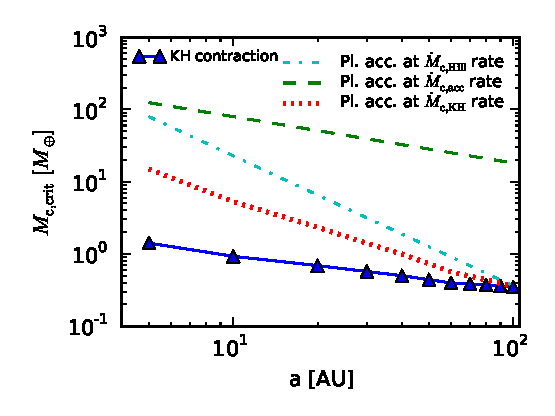
\includegraphics[width=0.5\textwidth]{../../figs/ModelAtmospheres/RadSelfGravRealEOS/PaperFigs/Mc_vs_a_poly_comp.pdf}
%\vspace{-0.5in}
\caption{Comparison between the critical core mass $M_{\rm{crit, KH}}$ given significant planetesimal accretion and the critical core mass when gas contraction dominates. Our results yield lower core masses than in the fast planetesimal accretion case (e.g., \citealt{rafikov06}). The critical core mass corresponding to $\dot{M}_{\rm c, Hill}$ and $\dot{M}_{\rm c, acc}$ from Figure \ref{fig:accrates} is plotted for comparison.}
\label{fig:raf2}
\end{figure}

The critical core mass in the regime where KH contraction dominates is smaller than in the case in which planetesimal accretion dominates the evolution of the atmosphere. This leads to two conclusions:

\begin{enumerate}
\item Planetesimal accretion can be safely ignored in our regime.
\item Giant planets can form from smaller cores if planetesimal accretion significantly reduces during atmosphere growth. 
\end{enumerate}

As additional heating due to planetesimals limits the atmosphere's ability to cool, our result represents a true minimum for the core mass needed to form a gas giant during the lifetime of the protoplanetary disk.


% First, we confirm that planetesimal accretion can be safely ignored in our regime of interest. Secondly, this comparison tells us that the core mass needed to form a giant planet is smaller if the core forms first, then accretes a massive envelope, than in the case where the core and atmosphere grown simultaneously in a high planetesimal accretion regime. Moreover, our result represents a true, absolute minimum on the core mass needed to form a giant planet during the lifetime of the protoplanetary disk, as our core no longer grows.


 \section{Summary}
 \label{conclusions}
 
 In this paper we study the formation of giant planets embedded in a gas disk. We consider atmosphere evolution around fully grown cores and determine the minimum (critical) core mass required to form a gas giant during the typical lifetime of a protoplanetary disk. We improve the model developed in Piso \& Youdin (submitted, hereafter Paper I) by including realistic equation of state (EOS) tables and dust opacities. 
 
 For a realistic EOS and grain growth opacity with maximum particle size $a_{\rm max}=1$ cm and a power-law size distribution (\ref{eq:graindistr}) with $p=3.5$, the critical core mass is $\sim$$7 M_{\oplus}$ at 5 AU in our fiducial disk and drops to $\sim$$4.5 M_{\oplus}$ at 100 AU. This result for the critical core mass $M_{\rm crit}$ is similar to the one obtained in Paper I for an ideal gas polytropic EOS and interstellar opacity. The realistic EOS and grain growth opacity have two competing effects on $M_{\rm crit}$:
 
 \begin{itemize}
 \item Realistic EOS effects increase $M_{\rm crit}$ by a factor of $\sim$$2$ when compared to the ideal gas polytrope.
 \item Grain growth opacities decrease $M_{\rm crit}$ by a factor of $\sim$$3$ at 5 AU and by a factor of $\sim$$1.5$ at 100 AU, when compared to ISM opacities, for a particle distribution given by the power-law (\ref{eq:graindistr}) with $p=3.5$ and a maximum particle size of 1 cm. The critical core mass is less sensitive to the location in the disk when realistic opacities are used. If $p=2.5$, an approximation for coagulation,  $M_{\rm crit}$ further reduces. 
 \end{itemize}
 
  
 %interstellar grain opacity, the critical core mass is $\sim$$20 M_{\oplus}$ at 5 AU and drops to $\sim$$6 M_{\oplus}$ in our fiducial disk. These results are more than twice as large than those calculated in Paper I for a polytropic EOS, and bring the critical core mass to $\sim$$10 M_{\oplus}$, the value typically quoted in many core accretion studies. When realistic opacities that include grain growth are used, the critical core mass is significantly lower, i.e. $\sim$$6 M_{\oplus}$ at 5 AU and $\sim$$4 M_{\oplus}$ at 100 AU. Different assumptions about the grain size distribution (e.g., that take into account coagulation) may further reduce the critical core mass.
 
Our results yield lower core masses than analogous results that consider high planetesimal accretion rates for which the core and atmosphere grow simultaneously. It is thus possible to form a giant planet from a smaller core if the core grows first, then the accretion rate of solids is reduced and a gaseous envelope is accumulated. Moreover, since additional heat sources such as planetesimal accretion limit the ability of the atmosphere to cool and undergo Kelvin-Helmholtz contraction, our results represent a true minimum on the core mass needed to form a giant planet during the typical lifetime of a protoplanetary disk.
 
  
% In this paper we study giant planet formation assuming that planetesimal accretion is negligible and the atmosphere evolution is dominated by KH gas contraction. We use the model developed in Paper I to determine the critical core mass to form a giant planet before disk dissipation assuming that the nebular gas obeys a realistic EOS that takes into account non-ideal effects. We find that variations in the adiabatic gradient due to thermodynamic effects such as dissociation and hydrogen spin isomers result in a critical core mass more than twice as large than in the case of a gas described by an ideal gas polytrope. This brings the critical core mass to $M_{\rm{c, crit}} \sim 10 M_{\oplus}$, which is the value typically quoted in many core accretion studies (see PY 13). We further make realistic assumptions about the dust opacity in the protoplanetary disk by taking into account grain growth. The resulting critical core mass is much less sensitive to outer boundary conditions (disk temperature and pressure) and is found to be $M_{\rm{c, crit}} \sim 5 M_{\oplus}$. Different grain size distribution assumptions (i.e., that take into account coagulation) may further reduce the critical core mass.
  
 %While for an ideal diatomic gas the minimum core mass to form a giant planet under the assumptions of our model is lower than the typically quoted value of $10 M_{\oplus}$ (see PY13), the inclusion of non-ideal effects brings this values back to around $10 M_{\oplus}$
 
% We also compare our results to studies that assume high planetesimal accretion rates, due to which the atmosphere is in steady state and entirely heated by planetesimals, and find that that our model yields lower critical core masses. This shows that it is easier to form a giant planet by growing the core first, then reducing the planetesimal accretion rate and letting the atmosphere evolve on a KH time scale. Moreover, since additional heat sources such as planetesimal accretion limit the ability of the atmosphere to cool and undergo KH contraction, our results represent a true minimum on the core mass needed to form a giant planet during the typical lifetime of a protoplanetary disk.
 
% In this paper we have studied the formation of giant planet atmospheres under the assumption that Kelvin-Helmoholtz gas contraction dominates the luminosity evolution of the atmosphere over planetesimal accretion. We built quasi-static two-layer atmosphere models with an inner convective region and an outer radiative region that matches smoothly onto the protoplanetary disk. We derived a cooling model to connect series of quasti-static atmospheres, and thus obtained an evolutionary history of the envelope. We defined the time at which unstable atmosphere collapse commences as $M_{\rm atm}(t)\sim M_{\rm c}$. From this we defined as ``critical core mass'' the minimum core mass for a protoplanet to initiate runaway gas accretion during the lifetime of the protoplanetary disk. We studied this minimum mass for a variety of disk conditions, nebular gas compositions and opacities. We found that the critical core mass decreases as we move further out in the disk, and is smaller for lower disk temperatures and opacities and for higher mean molecular weight of the gas. 
% 
% We find that the critical core mass to form a giant planet within the life time of the disk is smaller than the results yielded by studies that assume that the atmosphere evolution is dominated by the luminosity due to planetesimal accretion. We have showed that the planetesimal accretion rate needed to grow the core on a typical disk time scale is larger than the expected planetesimal accretion rates at large separations. As such, it is faster to form a planet by growing the core first in a fast planetesimal accretion regime (e.g., the core forms in the inner disk, then migrates outwards), then significantly reduce planetesimal accretion and allow a massive atmosphere to accumulate. 
 
%Our study assumes that the protoplanetary core forms first, then it r
 
%---------------------------------------------------------------------------

\acknowledgements{We thank Sean Andrews for providing us with the \citet{dalessio01} opacity tables. We also thank Eugene Chiang and Steven Cranmer for useful conversations. ANY thanks Phil Arras for a methodical explanation of entropy.}

\bibliographystyle{apj}
\bibliography{refs}

\appendix
\section{Equation of State Tables}\label{EOStables}

In this study we consider atmosphere growth in the outer parts of protoplanetary disks ($5<a<100$ AU), where temperature and pressure drop to as little as $T \sim 20$ K and $P \sim10^{-4}$ dyn cm$^{-2}$ for our MMSN disk model (see equations \ref{eq:diskb} and \ref{eq:Pd}). We assume that the nebular gas is described by a realistic equation of state (EOS), as prescribed by the \citet{saumon95} EOS tables. However, these tables only cover a relatively high range of temperatures and pressures, i.e. $2.1 < \log_{10} T(\rm{K})<7.06$ and $4.0<\log_{10}P$(dyn cm$^{-2})<19.0$. We thus need to extend the tables to lower $T$ and $P$, as required by our disk model. We calculate $\delad$ for

\begin{eqnarray}
1.0 & < & \log_{10} T <2.1 \\ 
-4.4& < & \log_{10} P<4.0 \\
\end{eqnarray} 
using the following method.



%In this section we explain the procedure for extending and interpolating the \cite{saumon95} EOS tables. The EOS takes into account non ideal interactions, and includes physical treatments of dissociation and ionization. However, the \cite{saumon95} EOS tables only cover a relatively high range of temperatures and pressures: $2.10 < \log_{10} T(\rm{K})<7.06$ and $4<\log_{10}P$(dyn cm$^{-2})<19$. We consider cold disks, where the temperature and pressure drop to $\sim 20$ K and $\sim 10^{-4}$ dyn cm$^{-2}$, respectively (see equations (\ref{eq:diskb}) and (\ref{eq:Pd})). It is therefore necessary to extend the \cite{saumon95} EOS tables to lower temperature and pressure values.

%We choose $\log_{10} T (\rm{K})=1$ and $ \log_{10}P$(dyn cm$^{-2})=-4.4$ as our lower boundaries for temperature and pressure, respectively. Our temperature and pressure grid becomes: $1 < \log_{10} T(\rm{K})<7.06$ and $-4.4<\log_{10}P$(dyn cm$^{-2})<19$. The other thermodynamic variables in the tables are calculated as follows.

\subsection{Hydrogen}

\label{hydrogen}

For a system of particles, the partition function can be written as the product of all partition functions associated with each type of internal energy:

%\begin{equation}
%\label{eq:z}
%Z=Z_t Z_r Z_v Z_e Z_n,
%\end{equation}

\begin{equation}
\label{eq:zagain}
Z=Z_t Z_r Z_v
\end{equation} 

\noindent where $Z_t$, $Z_r$, $Z_v$ are the partition functions associated with translation, rotation, and vibration, respectively. \footnote{We ignore electronic and nuclear excitation as they are only important at temperatures much higher than our regime of interest.} Our derivations follow \citet{kittel} %For hydrogen, electronic and nuclear excitation are only significant at temperatures higher than our region of interest ($\theta_e \approx 12000$ K and $\theta_n >> \theta_e$, where $\theta_e$ and $\theta_n$ are the characteristic temperatures for electronic and nuclear excitation, respectively). As such, we will only take into account the translation, rotation and vibration of the hydrogen molecule:

%In what follows we present and briefly derive expressions for thermodynamic variables based on quantum mechanics principles. More details on the derivations can be found in \citet{kittel}.

In the classical limit, the partition function associated with the motion of the center of mass of a gas molecule of mass $m$ is given by:

\begin{equation}
\label{eq:Zt}
Z_t=(m/2 \beta \pi \hbar^2)^{3/2} V,
\end{equation}
with  $T$ and $V$ the gas temperature and volume, respectively, $\hbar$ the reduced Planck constant, and  $\beta=1/(k_b T)$. The rotational partition function is generally written as:

\begin{equation}
\label{eq:Zr}
Z_r=\sum_0^\infty (2 j+1) \exp{\Big[\frac{-j (j+1)\Theta_r}{T}\Big]},
\end{equation}

\noindent where $\Theta_r$ is the characteristic temperature for rotational motion. In the case of hydrogen, $\Theta_r \approx 85$ K. However, molecular hydrogen occurs in two isomeric forms: orthohydrogen, with the proton spins aligned parallel to each other, and parahydrogen, with the proton spins aligned antiparallel. Parahydrogen can only a have symmetric (even) wave function associated with rotation, while orthohydrogen can only have an antisymmetric (odd) wave function associated with rotation. The rotational partition functions for ortho- and parahydrogen can thus be written as:

\begin{equation}
\label{eq:Zpara}
Z_{\rm{r,para}}=\frac{1}{2}\sum_0^\infty (1+(-1)^j) (2 j +1) \exp\Big[-\frac{j(j+1)\Theta_r}{T}\Big]
\end{equation}
and
\begin{equation}
\label{eq:Zortho}
Z_{\rm{r,ortho}}=\frac{3}{2}\sum_0^\infty (1-(-1)^j) (2 j +1) \exp\Big[-\frac{j(j+1)\Theta_r}{T}\Big]
\end{equation}
The factor of 3 in Equation (\ref{eq:Zortho}) accounts for the three-fold degeneracy of the ortho state.

 When the two isomers are in equilibrium, the combined partition function is given by the sum of the individual partition functions, $Z_{\rm r}=Z_{\rm{r, ortho}}+Z_{\rm{r,para}}$ and can be written as:

\begin{equation}
\label{eq:Zrspin}
Z_r=\sum_0^\infty (2-(-1)^j) (2j+1) \exp{\Big[\frac{-j (j+1) \Theta_r}{T}\Big]}
\end{equation}
In our range of temperatures of interest, we found that $Z_r$ converges after about 25 terms in the series.


Finally, the partition function for vibrational motion is given by:

\begin{equation}
\label{eq:Zv}
Z_v=[1-\exp{(\theta_v/T)}]^{-1},
\end{equation}

\noindent where $\theta_v$ is the characteristic temperature for vibrational motion, $\theta_v \approx 6140$ K for hydrogen. 

If the partition function of a system particles is known in terms of $(V, T)$, the internal energy per unit mass, entropy per unit mass and specific heat capacity can be written as

%\begin{equation}
%\label{eq:U}
%U_N=k T^2 \Big(\frac{\partial \log{Z}}{\partial T}\Big)_{V, N}
%\end{equation}
%
%\begin{equation}
%\label{eq:S}
%S_N=k \log{Z} + \frac{U_N}{T}
%\end{equation}
%
%The energy, and entropy per mass and specific heat capacity will subsequently be:

\begin{equation}
\label{eq:u}
U=\mathcal{R} T^2 \Big(\frac{\partial \log{Z}}{\partial T}\Big)_{V}
\end{equation}
\begin{equation}
\label{eq:s}
S=\mathcal{R} \log{Z} + \frac{U}{T}
\end{equation}
\begin{equation}
\label{eq:cv}
C_v=\Big(\frac{\partial U}{\partial T}\Big)_{V}.
\end{equation}
Since $Z=Z_t Z_r Z_v$, we may write $U=U_t+U_r+U_v$ and $S=S_t+S_r+S_v$, where $U_t$, $U_r$, $U_v$, $S_t$, $S_r$, $S_v$ are the quantities corresponding to the individual translation, rotation and vibration partition functions, respectively.

The entropy per mass due to translational motion can be expressed as:

\begin{equation}
\label{eq:st}
S_t=\mathcal{R} \Big[ \frac{5}{2} \ln{T} - \ln{P} + \ln \Big( \frac{(2 \pi)^{3/2} \mathcal{R}^{5/2} \mu^4}{h^3}\Big) +\frac{5}{2} \Big]
\end{equation}

\noindent with $\mu$ the mean molecular weight. Equation (\ref{eq:st}) is known as the Sackur-Tetrode formula, and it is only applicable to an ideal gas. The internal energy per mass due to translational motion is given by:

\begin{equation}
\label{eq:ut}
U_t=\frac{3}{2} \mathcal{R} T
\end{equation}

Putting all of the above together, we can now evaluate the thermodynamic quantities needed to extend the \cite{saumon95} EOS tables to low temperatures and pressures.

\begin{enumerate}

\item{\textbf{Density.}} In the low temperature, low pressure regime, hydrogen is molecular and behaves like an ideal gas. As such, the density in this region follows the ideal gas law $P=\rho \mathcal{R} T$.
\item{\textbf{Internal energy per mass.}} $U=U_t+U_r+U_v$, where $U_t$ is given by Equation(\ref{eq:ut}), and $U_r$ and $U_v$ are determined using equations (\ref{eq:u}), (\ref{eq:Zrspin}) and (\ref{eq:Zv}) above.
\item{\textbf{Entropy per unit mass}}. Similarly, $S=S_t+S_r+S_v$, where $S_t$ is given by Equation (\ref{eq:st}), and $S_r$ and $S_v$ can be determined from Equation (\ref{eq:s}) and the calculated expressions for $U_r$ and $U_v$, respectively.
\item{\textbf{Entropy logarithmic derivatives}}. The logarithmic derivatives $S_T$ and $S_P$ are given by:

\begin{equation}
\label{eq:sT}
S_T=\frac{\partial \log{S}}{\partial \log{T}} \Big |_P
\end{equation}
and
\begin{equation}
\label{eq:sP}
S_P=\frac{\partial \log{S}}{\partial \log{P}} \Big |_T
\end{equation}
We calculate $S_T$ and $S_P$ through finite differencing. 

\item{\textbf{Adiabatic gradient $\delad$}}. The adiabatic gradient is defined as:

\begin{equation}
\label{eq:deladSP}
\delad=\frac{\partial \log{T}}{\partial \log{P}} \Big |_S = -\frac{S_P}{S_T}
\end{equation}

We evaluate it from the tabulated values for $S_T$ and $S_P$ determined above. Figure \ref{fig:deladH} shows a contour plot of $\delad$ as a function of temperature and pressure for the extended EOS table.    %Our extension smoothly matches the original tables for $8.80<\log{S}$(K g$^{-1})<9.07$ (\textbf{numbers are wrong, change once you have the final figure version}).

\end{enumerate}

\begin{figure}[h!]
\centering
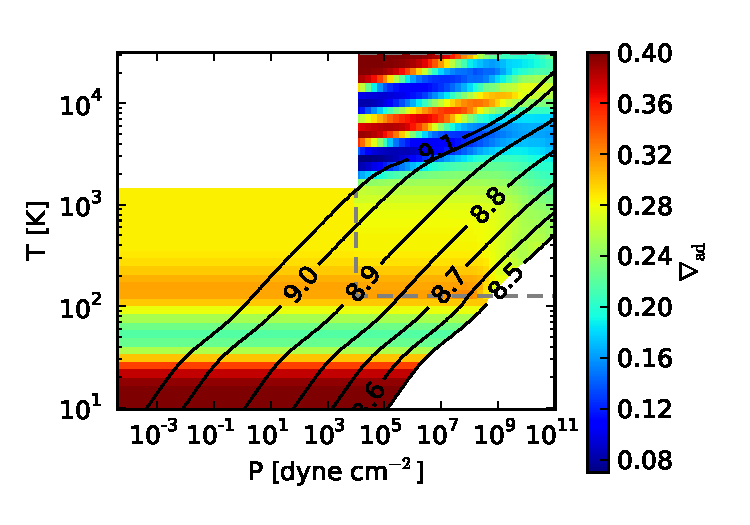
\includegraphics[scale=.8]{../../figs/ModelAtmospheres/RadSelfGravRealEOS/PaperFigs/delad_S_H.pdf}
\caption{Contour plot of the hydrogen adiabatic gradient $\delad$ as a function of gas temperature and pressure. The upper right rectangle encloses the region described by the original \citet{saumon95} EOS tables, while the rest of the plot is our extension to lower temperatures and pressures. The black curves represent constant entropy adiabats, with the labels the natural logarithm of the absolute entropy per unit mass. At high temperatures, hydrogen dissociates and ionizes, while at low temperatures the rotational states of the hydrogen molecule are only partially excited and it no longer behaves like an ideal diatomic gas. Regions in which the EOS is invalid or has not been computed are masked in white (see Figure \ref{fig:deladmap} caption for an explanation).}
\label{fig:deladH}
\end{figure}

\subsection{Helium}

We extend the helium EOS tables based on a similar procedure. Since helium is primarily neutral and atomic at low temperatures and pressures, we treat it as an ideal monoatomic gas, and thus only take into account the translational component of the partition function (\ref{eq:Zt}). Figure \ref{fig:deladHe} shows $\delad$ as a function of temperature and pressure for the extended EOS table. %The original and extended table join smoothly for entropy curves between $8.29<\log{S}$(K g$^{-1})<8.77$ in this case (\textbf{numbers are wrong, change once you have the final figure version}).

\begin{figure}[h!]
\centering
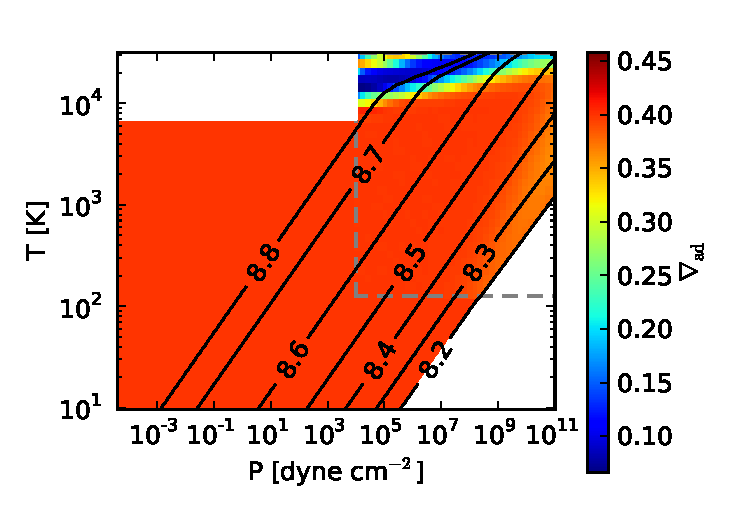
\includegraphics[scale=.8]{../../figs/ModelAtmospheres/RadSelfGravRealEOS/PaperFigs/delad_S_He.pdf}
\caption{Contour plot of the helium adiabatic gradient $\delad$ as a function of gas temperature and pressure. The upper right rectangle encloses the region described by the original \citet{saumon95} EOS tables, while the rest of the plot is our extension to lower temperatures and pressures. The black curves represent constant entropy adiabats, with the labels the natural logarithm of the absolute entropy per unit mass. Helium ionizes at $T \gtrsim 10,000$ K, but behaves as an ideal monatomic gas otherwise. We choose $T=7,000$ K as a conservative temperature cutoff above which our extension is no longer valid (masked in white). The EOS has not been computed in the lower-right region of the plot --- see Figure \ref{fig:deladmap} for an explanation.}
\label{fig:deladHe}
\end{figure}

\vspace{0.2in}

Lastly, we combine Figures \ref{fig:deladH} and \ref{fig:deladHe} to obtain the EOS tables for the hydrogen-helium mixture thorough the procedure described in \citet{saumon95}, for a helium mass fraction $Y=0.3$ (Figure \ref{fig:deladmap}).

%Using equation (\ref{eq:upartition}) we therefore recover the standard result $U_{\rm r}=\mathcal{R} T$ (refs). Furthermore, we know that the internal energy and entropy per unit mass associated with translation are given by $U_{\rm t}=\frac{3}{2} \mathcal{R}$ and $C_{\rm{v,t}}=\frac{3}{2}\mathcal{R}$, respectively, and so we are able to calculate the total internal energy and specific heat of a diatomic molecule as a function of temperature. An example of the variation of heat capacity with temperature is shown in \citet{kittel}, chapter 3. 

%The partition function associated with rotation is generally written as:
%
%\begin{equation}
%\label{eq:Zr}
%Z_{\rm r}=\sum_0^\infty (2 j +1) \exp\Big[-\frac{j(j+1)\Theta_r}{T}\Big],
%\end{equation}
%with $j$ the angular momentum quantum number \citep{kittel}. Various thermodynamic quantities can be derived from the partition function. For example, the internal energy per unit mass can be written as:
%
%\begin{equation}
%\label{eq:upartition}
%u_{\rm r}=\mathcal{R}T^2 \frac{\partial \log Z}{\partial T}
%\end{equation}
%
%The specific heat at constant volume then easily follows as
%
%\begin{equation}
%\label{eq:cvpartition}
%c_{\rm{v,r}}=\Big(\frac{\partial u}{\partial T}\Big)_V
%\end{equation} 


 





\section{Adiabatic Gradient Variations}
\label{alldelad}

\subsection{Adiabatic Gradient during Partial Dissociation}\label{deladdiss}

%The adiabatic gradient during dissociation or ionization is a function of temperature and the dissociation or ionization fraction $x$. The Saha equation (e.g., \citealt{kippenhahn90}) relates $x$ to the gas 


The total internal energy of a partially dissociated gas includes contributions from the individual internal energies of the molecules and atoms, as well as from the dissociation energy. The dissociation energy depends on the dissociation fraction $x$ (i.e., the fraction of molecules that have dissociated), which can be found from the Saha equation (see e.g., \citealt{kippenhahn90}, Chapter 14) as a function of temperature and density,

\begin{equation}
\label{eq:saha}
\frac{x^2}{1-x} \propto \frac{T^{3/2}}{\rho} e^{-\chi/k_B T},
\end{equation} 
where $\chi$=4.48 eV is the dissociation energy for molecular hydrogen \citep{blanksby03}.

The above also holds true for ionization, with the dissociation energy replaced by ionization energy $\chi=13.6$ eV for atomic hydrogen \citep{mandl89}. From the Saha equation one can find an expression for $\rho$ as a function of $T$ and $x$, then derive the adiabatic gradient directly from its definition (Equation \ref{eq:delad}), taking into account the fact that the mean molecular weight in the ideal gas law varies with $x$, hence the pressure will not only be a function of $T$ and $\rho$ but also of $x$ (see \citealt{kippenhahn90}, Chapter 14.3 for a detailed derivation). The final expression for the adiabatic gradient during ionization is 

\begin{equation}
\label{eq:deladioniz}
\delad=\frac{2+x (1-x) \Phi_H}{5+x(1-x)\Phi_H^2},
\end{equation}
with $\Phi_H \equiv \frac{5}{2}+\frac{\chi}{k_B T}$. The derivation of $\delad$ during dissociation is more involved mathematically (see, e.g., \citealt{vardya60}) and leads to a slightly more complicated final expression,

%One can derive a simple expression for the adiabatic gradient as a function of $x$ and $T$ from it's definition (equation \ref{eq:delad}), using the 

%The adiabatic gradient follows as (see \citealt{vardya60} for a detailed derivation)

\begin{equation}
\label{eq:deladdiss}
\delad=\frac{1+x+ \frac{x(1-x^2)}{2} \frac{\chi}{k_B T}}{5 x + \frac{7(1-x)}{2} + \frac{x(1-x^2)}{2} \Big(\frac{\chi}{k_B T}\Big)^2} \, .
\end{equation} 
Using Equation (\ref{eq:deladdiss}), we recover $\delad=2/7$ for $x=0$ (no ongoing dissociation hence hydrogen is purely molecular and diatomic) and $\delad=2/5$ for $x=1$ (hydrogen is fully dissociated into atoms and hence monatomic). Figure \ref{fig:deladdiss} shows the dependence of $\delad$ on the dissociation fraction, for $T=3000$ K, the temperature at which dissociation typically occurs \citep{langmuir12}. The adiabatic gradient drops substantially during partial dissociation, since part of the internal energy is used in dissociation rather than in increasing the temperature of the system.


\begin{figure}[h]
\centering
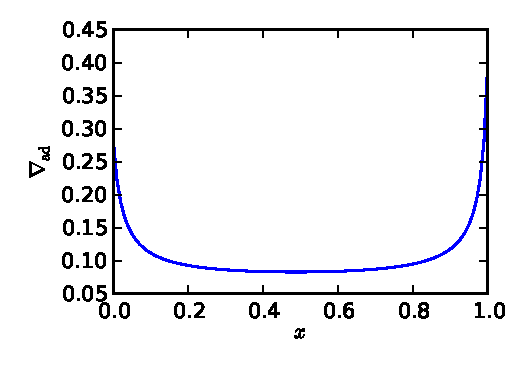
\includegraphics[width=0.5\textwidth]{../../figs/ModelAtmospheres/RadSelfGravRealEOS/PaperFigs/delad_dissociation.pdf}
%%\vspace{-0.5in}
\caption{Adiabatic gradient as a function of the hydrogen dissociation fraction $x$. The adiabatic gradient is $\delad=2/7$ for pure molecular hydrogen ($x=0$) and $\delad=2/5$ for fully atomic hydrogen ($x=1$), and drops to low values during partial dissociation.}
\label{fig:deladdiss}
\end{figure}


\subsection{Adiabatic Gradient during Conversion of Spin Isomers}
\label{deladspin}

The adiabatic gradient scales as $\delad \sim 1/c_{\rm V}=1/(c_{\rm V,t}+c_{\rm V,r}) \sim 1/c_{\rm V, r}$, where $c_{\rm V}$ is the specific heat capacity at constant volume, and $c_{\rm V, t}$ and $c_{\rm V,r}$ are the translational and rotational components, respectively. The second equality is due to the fact that $c_{\rm V, t}=3\mathcal{R}/2$ is independent of temperature . We can therefore understand how conversion between spin isomers affects $\delad$ by studying the dependence on temperature of $c_{\rm V, r}$ of the ortho-para mixture. 

The internal energy per unit mass and specific heat capacity associated with rotation for the individual isomers and for the equilibrium mixture can be derived from their partition functions (see \App{EOStables} for details), and are plotted in Figure  \ref{fig:ucvr} (after \citealt{farkas35}, Figure 1). At low temperatures, parahydrogen is in the $j=0$ state and has no rotational energy, while orthohydrogen is in the $j=1$ state and has the energy of its first rotational level. Both para- and orthohydrogen, as well as their equilibrium mixture, behave like monatomic gases at low temperatures and thus have zero rotational heat capacity. This is consistent with $\delad=2/5$ at low temperatures as seen in Figure \ref{fig:deladmap}. As the temperature increases, the energetically higher-lying rotational states of para- and orthohydrogen are populated and the heat capacity of both spin isomers increases as a result. We note that the heat capacity of the equilibrium mixture is not a weighted average of the heat capacities of the individual components because it takes into account both the rotational energy uptake of para- and orthohydrogen, and also the shift in their equilibrium concentrations with temperature. This results in a peak in the heat capacity of the mixture around $\sim$$50$ K, as seen in the bottom plot of Figure \ref{fig:ucvr}. As $\delad \sim 1/c_{\rm{V,r}}$, it follows that the adiabatic gradient has to reduce, reach a minimum, then increase as the temperature rises, as shown in Figure \ref{fig:deladmap}.

% As the temperature increases, the energetically higher-lying ($j=1$) ortho-hydrogen is formed, and the concomitant energy increase is seen as a peak in the heat capacity of the equilibrium mixture. 


%There are two significant maxima in the heat capacities of parahydrogen and of the mixture. At very low temperatures, the heat capacity of parahydrogen is zero because only the lowest accessible energy level $j=0$ is occupied and a temperature increase does not provide enough energy to populate the next higher level. When the temperature becomes sufficiently high to populate the second lowest level $j=2$, the heat capacity rapidly increases, passes through a maximum and starts to decrease when the second lowest level becomes saturated. 


%the adiabatic gradient is inversely proportional to the heat capacity, it 

%means that  the former has to first decrease from 2/5 as the temperature increases, reach a minimum around 50 K ($\delad \approx 0.25$ from Fig. \ref{fig:deladmap}), then gradually increase to 2/7 as for a diatomic gas. This behavior is illustrated in Figure \ref{fig:deladmap}.  



%The maxima in the ortho-para mixture appears when parahydrogen starts converting into orthohydrogen. The heat capacity of the equilibrium mixture is not a weighted average of the heat capacities of the individual components because it takes into account both the rotational energy uptake of para- and orthohydrogen, and also the shift in their equilibrium concentrations with temperature. At $T=0$, only parahydrogen is present in the equilibrium mixture; as the temperature is increased, the energetically higher-lying ($j=1$) ortho-hydrogen is formed, and the concomitant energy increase is seen as a peak in the heat capacity. As the adiabatic gradient is inversely proportional to the heat capacity, it means that  the former has to first decrease from 2/5 as the temperature increases, reach a minimum around 50 K ($\delad \approx 0.25$ from Fig. \ref{fig:deladmap}), then gradually increase to 2/7 as for a diatomic gas. This behavior is illustrated in Figure \ref{fig:deladmap}.  



\begin{figure}[h]
\centering
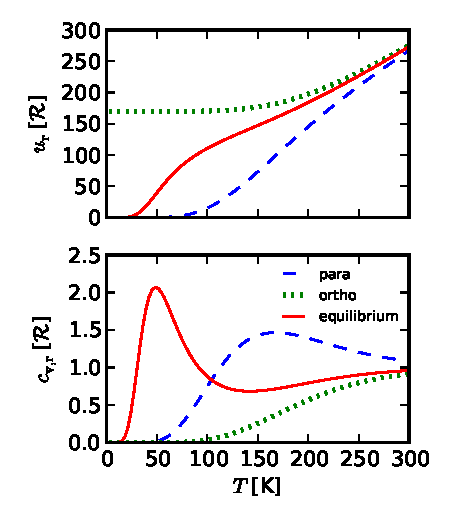
\includegraphics[width=0.5\textwidth]{../../figs/ModelAtmospheres/RadSelfGravRealEOS/PaperFigs/ortho_para_energy.pdf}
%%\vspace{-0.5in}
\caption{Internal energy per unit mass and specific heat capacity associated with rotation for parahydrogen (dashed blue), orthohydrogen (dotted green), and the equilibrium mixture (solids red) as a function of temperature. After \citet{farkas35}, Figure 1.}
\label{fig:ucvr}
\end{figure}


%with $\chi$ and $T$ the dissociation energy and temperature, respectively, equal to $\chi=4.48$ eV\citep{blanksby03} and $T\sim3000$ K \citep{langmuir12} for molecular hydrogen.

%Specifically, if we denote the internal energies of neutral hydrogen, protons and electrons as $U_{H}$, $U_+$ and $U_e$, respectively, then the total internal energy of the gas is given by:

%\begin{equation}
%U=U_H+U_+ + U_e + x \chi,
%\end{equation}
%
%\noindent where $x$ is the ionization fraction and $\chi$ is the ionization energy (equal to -13.6 eV for hydrogen). The ionization fraction can be determined from the Saha equation (see e.g., \citealt{kippenhahn90}).
%
%\begin{equation}
%\label{eq:saha}
%\frac{x^2}{1-x} \frac{\rho}{m_H}=\frac{(2 \pi m_e k_B T)^{3/2}}{h^3} e^{-\chi/k_B T},
%\end{equation}
%
%\noindent where $m_e$ is the mass of the electron and $h$ is Planck's constant. It can be seen from the Saha equation that the ionization fraction depends only on the gas temperature and density: $x=x(T, \rho)$. As such, all the thermodynamic quantities also depend only on the gas temperature and density, and hence on the equation of state. The adiabatic gradient is given by (see \citealt{kippenhahn90}, chapter 14 for a derivation):
%
%\begin{equation}
%\delad=\frac{2+x (1-x) \Phi_H}{5+x (1-x) \Phi_H^2},
%\end{equation} 
%with $\Phi_H=\frac{5}{2}+\frac{\chi}{k T}$. Figure \ref{fig:deladion} shows the behavior of $\delad$ for partially ionized hydrogen. We recover $\delad=2/5$ for $x=0$ (pure atomic hydrogen) and $x=1$ (fully ionized plasma). The adiabatic gradient decreases significantly for intermediate values of $x$, becoming smaller than 0.1 at its minimum (for $x=0.5$). 

\section{Grain growth opacity and radiative windows} \label{radwindow}

The opacity of the interstellar medium is reasonably well constrained and approximate analytic expressions for the Rosseland mean opacity as a function of temperature and density are derived in \citet{bell94}. For low temperatures ($T \lesssim 100$ K) at which ice grains are present, opacity scales with temperature as $\kappa \sim T^2$. Sublimation of ice grains at $\sim$$150$ K and of metal grains at $\sim$$1000$ K results in sharp opacity drops. This is shown in Figure \ref{fig:opacity} for a gas density $\rho=10^{-8}$ g cm$^{-3}$, which is typical for the outer regions of protoplanetary disks. \citet{semenov03} calculate Rosseland mean opacities in protoplanetary disks for grains of different sizes and structure. As shown in Figure \ref{fig:opacity}, their results are in good agreement with \citet{bell94}. However, \citet{semenov03} do not take grain growth into account, which is likely to occur in protoplanetary disks, particularly at the late times when cores form. \citet{dalessio01} compute wavelength dependent opacities for a range of maximum particle sizes and different size distributions. Figure \ref{fig:opacity} shows the integrated Rosseland mean opacity for a maximum particle size of 1 cm and a power law size distribution $n \sim a^{-p}$, with $a$ the grain size and $p=3.5$ for a normal collisional cascade and $p=2.5$ when coagulation is taken into account. We see in Figure \ref{fig:opacity} that this yields a mean opacity that is both lower and less sensitive to temperature, when compared to \citet{bell94} or \citet{semenov03}. However, observations of dust in protoplanetary disks have only been made at low temperatures (i.e., before dust sublimates). As we see in Figure \ref{fig:opacity}, the opacity dramatically decreases during dust sublimation for ISM grains, which can result in regions in the inner parts of planetary atmospheres where energy is transported radiatively, i.e. radiative windows. We thus use the \citet{bell94} opacities for $T \gtrsim 1000$ K, ensuring that they smoothly match the \citet{dalessio01} opacities for lower temperatures.

\begin{figure}[h!]
\centering
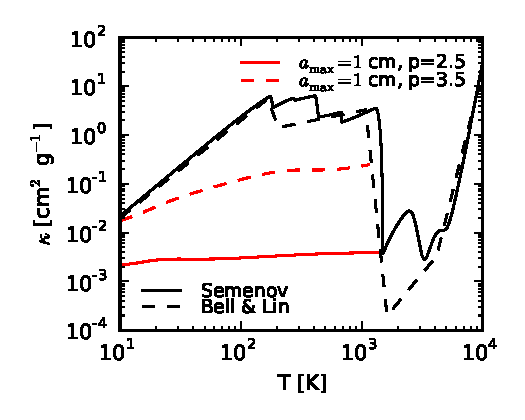
\includegraphics[width=0.5\textwidth]{../../figs/ModelAtmospheres/RadSelfGravRealEOS/PaperFigs/kappa_grain_growth_SBL_paper.pdf}
%%\vspace{-0.5in}
\caption{Rosseland mean opacity of dust grains as a function of temperature for different opacity assumptions. The dashed black curve shows the \citet{bell94} analytic ISM opacity for $\rho=10^{-8}$ g cm$^{-3}$. The solid black curve shows the tabulated opacity of \citet{semenov03} for a dust composition of 'normal' silicates. The dashed red curve shows the \citet{dalessio01} opacity, which takes grain growth into account, for a maximum particle size of 1 cm and a standard collisional cascade grain size distribution ($p=3.5$). The solid red curve is the same as the dashed red curve, but it accounts for coagulation ($p=2.5$).}
\label{fig:opacity}
\end{figure}

The significant opacity drop due to the sublimation of ice and metal grains lowers the radiative temperature gradient $\delrad$, which may result in one or more inner radiative layers inside the atmosphere of a protoplanet. This is displayed in Figure \ref{fig:delvsr}: depending on the semimajor axis and core mass, the opacity drop will generate no radiative window (top panel), one radiative window (middle panel), or two radiative windows (bottom panel). 

\begin{figure}[h!]
\centering
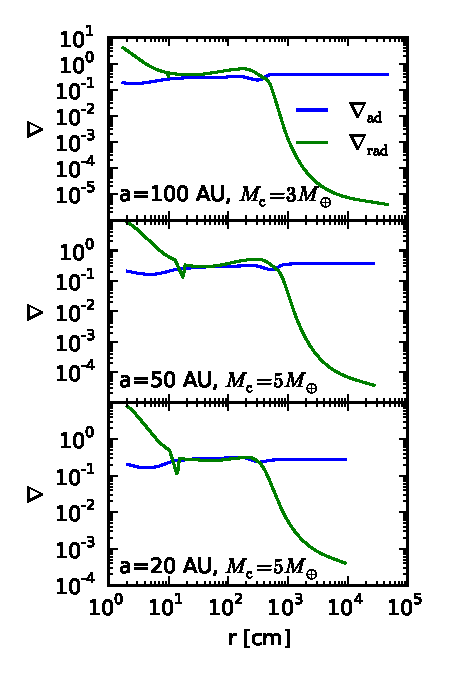
\includegraphics[width=0.5\textwidth]{../../figs/ModelAtmospheres/RadSelfGravRealEOS/PaperFigs/del_vs_r.pdf}
%%\vspace{-0.5in}
\caption{Snapshots of the radiative and adiabatic gradient as a function of the radial coordinate, for planets with different core masses forming at various locations in the disk. The nebular gas is described by a realistic EOS. The sharp drop in opacity due to dust sublimation may generate one or more radiative windows. Top panel: no radiative window for $a=100$ AU and $M\co=3 M_{\oplus}$. Middle panel: the sharp opacity decrease produces one radiative window for $a=50$ AU and $M\co=5 M_{\oplus}$. Bottom panel: the decrease in opacity results in two radiative windows for $a=20$ AU and $M\co=3 M_{\oplus}$.}
\label{fig:delvsr}
\end{figure}



\end{document}




